\documentclass{article}

\usepackage{PRIMEarxiv}

\usepackage[utf8]{inputenc} % allow utf-8 input
\usepackage[T1]{fontenc}    % use 8-bit T1 fonts
\usepackage{hyperref}       % hyperlinks
\usepackage{url}            % simple URL typesetting
\usepackage{booktabs}       % professional-quality tables
\usepackage{amsfonts}       % blackboard math symbols
\usepackage{nicefrac}       % compact symbols for 1/2, etc.
\usepackage{microtype}      % microtypography
\usepackage{fancyhdr}       % header
\usepackage{graphicx}       % graphics
\graphicspath{{media/}}     % organize your images and other figures under media/ folder

% Math and theorem environments
\usepackage{amsmath,amssymb,amsthm,bm}
\usepackage{tikz}
\usepackage{xcolor}
\usepackage{tcolorbox}
\tcbuselibrary{skins,breakable}
\definecolor{personalcontribcolor}{RGB}{30,136,229}
\definecolor{k3color}{RGB}{233,30,99}

% Header
\pagestyle{fancy}
\thispagestyle{empty}
\rhead{ \textit{} }

% Update your Headers here
\fancyhead[LO]{Low-rank random features and NTK}

% Macros
\DeclareRobustCommand{\ReLU}{\mathrel{\boldsymbol{\sigma}}}



\newcommand{\Kop}{\boldsymbol{\Theta}}
\newtheorem{theorem}{Theorem}
\newtheorem{proposition}{Proposition}
\newtheorem{assumption}{Assumption}

%% Title
\title{The landscape of random features low rank neural networks}

\author{
  Janis Aiad\thanks{First author, work done during a visit at UMD}$^{1}$ \and Haizhao Yang$^{2}$ \and Shijun Zhang$^{3}$ \\
  $^{1}$ École Polytechnique \\
  $^{2}$ University of Maryland, Department of Mathematics; Department of Computer Science \\
  $^{3}$ The Hong Kong Polytechnic University
}

\begin{document}
\maketitle

\begin{abstract}
We study low-rank random feature models (MMNN), an architecture where only the linear outputs \( A^{(\ell)} \) are trained while the input weights \( w^{(\ell)} \) are frozen at random. This factorization drastically reduces the parameter budget, enables mean-field analysis even at moderate widths (\( n \sim 500{-}5000 \)), and exhibits dictionary/wavelet-like feature learning. We connect MMNN training dynamics to (i) stepwise loss curves arising from band-by-band Fourier mode activation, analogous to multi-index learning; (ii) three-layer mean-field convergence via universal approximation holding at all finite times; and (iii) low-to-high frequency learning explained by kernel gradient flow in Fourier space. Numerical experiments reveal that MMNNs learn high-frequency spikes through recursive construction across layers, with depth directly correlating to maximal learned frequency. We formalize the simplified model without bias scaling, derive the NTK recursion, and explain how rank \( r \) bottlenecks yield \( O(1/r) \) kernel fluctuation decay and improved preconditioning.
\end{abstract}

% keywords can be removed
\keywords{Neural Tangent Kernel \and Mean-Field \and Random Features \and Low Rank \and Scaling Laws \and Infinite Width}

\tableofcontents

\vspace{2em}
\section{Introduction}
We consider low-rank random feature models (MMNN) as a principled architecture where at each layer \( \ell \), the network linearly combines a frozen random nonlinear basis, and only the output weights \( A^{(\ell)} \) are trained. This design choice yields three key advantages: (i) linear scaling of trainable parameters with width (parameter budget \( O(rn) \) vs \( O(n^2) \)), (ii) avoidance of Riemannian gradient descent issues from matrix factorization, and (iii) preservation of universal approximation via frozen random features with full support.

\paragraph{Motivation: scientific machine learning and PDE solvers.}
A central question in scientific machine learning is why low-rank random feature architectures achieve high regression accuracy despite having significantly fewer trainable parameters than fully-connected networks. Understanding this phenomenon is crucial for improving practical applications, particularly physics-informed neural networks (PINNs) and neural PDE solvers, where computational efficiency and the ability to learn high-frequency solutions are paramount. This paper develops a comprehensive theoretical framework to explain the loss landscape, training dynamics, and expressivity of low-rank random features, connecting three regimes: (i) early NTK-dominated lazy learning, (ii) mid-training mean-field dynamics with stepwise loss curves, and (iii) late-training sharp minima requiring careful optimization. By exposing the mechanisms behind why these architectures succeed—particularly their ability to learn hierarchical frequency representations and maintain global convergence guarantees—we aim to guide the design of more efficient neural network architectures for scientific computing applications where spectral accuracy and parameter efficiency are critical.

\paragraph{Fourier space interpretation and stepwise loss.}
Empirically, MMNN training exhibits stepwise (staircase-like) loss curves—long plateaus followed by sharp drops—reminiscent of multi-index learning dynamics~\cite{benarous2021online}. We propose that in Fourier space, the mean-field kernel gradient flow \( \partial_t f_t = -\Theta_t(f_t - f^*) \) diagonalizes into mode-wise exponential decay \( \partial_t \hat{e}_t(\omega) = -\kappa_t(\omega) \hat{e}_t(\omega) \), where \( \kappa_t(\omega) \) is the time-varying Fourier symbol of the kernel. Initially, only low-frequency modes have large \( \kappa_t(\omega) \), yielding rapid loss drop; as the feature distribution evolves via mean-field transport, \( \kappa_t(\omega) \) grows on higher \( |\omega| \), activating new spectral bands in stages. Each plateau corresponds to residual energy in modes with negligible \( \kappa_t(\omega) \); each drop corresponds to a band becoming active. This band-by-band activation explains the observed stepwise curves when only a small Fourier decomposition is effectively active at any time.

\begin{figure}[htbp]
    \centering
    \includegraphics[width=0.8\textwidth]{media/stepwise_training_dynamics.pdf}
    \caption{Stepwise training dynamics of MMNN. The training loss exhibits characteristic staircase behavior with plateaus (residual energy in inactive frequency bands) followed by sharp drops (activation of new frequency bands). Each phase corresponds to learning a different part of the Fourier spectrum, with low frequencies learned first and high frequencies activated sequentially through mean-field dynamics.}
    \label{fig:stepwise_intro}
\end{figure}

\paragraph{Three-layer mean-field convergence.}
Unlike two-layer analyses that exploit convexity, three-layer MMNN convergence relies on a universal approximation property holding at \emph{all finite training times}—not just at convergence~\cite{globalconvergencesthreelayer}. The frozen random features \( w^{(\ell)} \) maintain full support throughout training, ensuring the feature span remains dense and capable of capturing all Fourier content. The mean-field framework operates in moderate widths (\( n \sim 500{-}5000 \)), is dimension-agnostic (no curse of dimensionality from NTK high-dimensional statistics), and naturally explains the observed dictionary/wavelet learning where ReLU gating selects spike locations and frequencies recursively build across layers.

\subsection*{A motivating architecture and its two-layer NTK}
The considered architecture is:
\begin{figure}[htbp]
    \centering
    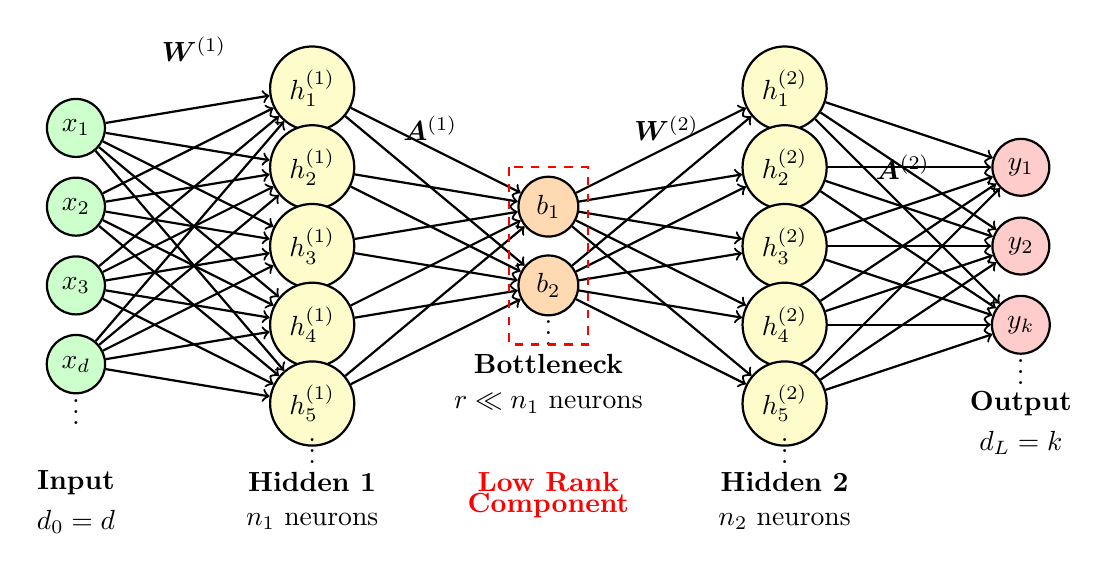
\begin{tikzpicture}[
        node distance=2cm and 3cm,
        neuron/.style={circle, draw, fill=blue!20, minimum size=15pt},
        input/.style={circle, draw, fill=green!20, minimum size=15pt},
        output/.style={circle, draw, fill=red!20, minimum size=15pt},
        hidden/.style={circle, draw, fill=yellow!20, minimum size=15pt},
        bottleneck/.style={circle, draw, fill=orange!30, minimum size=15pt},
        thick
    ]
    
    % Input layer
    \node[input] (x1) at (0,2) {$x_1$};
    \node[input] (x2) at (0,1) {$x_2$};
    \node[input] (x3) at (0,0) {$x_3$};
    \node[input] (xd) at (0,-1) {$x_d$};
    \node at (0,-1.5) {$\vdots$};
    
    % First hidden layer
    \node[hidden] (h11) at (3,2.5) {$h_1^{(1)}$};
    \node[hidden] (h12) at (3,1.5) {$h_2^{(1)}$};
    \node[hidden] (h13) at (3,0.5) {$h_3^{(1)}$};
    \node[hidden] (h14) at (3,-0.5) {$h_4^{(1)}$};
    \node[hidden] (h15) at (3,-1.5) {$h_5^{(1)}$};
    \node at (3,-2) {$\vdots$};
    
    % Bottleneck layer (low rank)
    \node[bottleneck] (b1) at (6,1) {$b_1$};
    \node[bottleneck] (b2) at (6,0) {$b_2$};
    \node at (6,-0.5) {$\vdots$};
    
    % Second hidden layer
    \node[hidden] (h21) at (9,2.5) {$h_1^{(2)}$};
    \node[hidden] (h22) at (9,1.5) {$h_2^{(2)}$};
    \node[hidden] (h23) at (9,0.5) {$h_3^{(2)}$};
    \node[hidden] (h24) at (9,-0.5) {$h_4^{(2)}$};
    \node[hidden] (h25) at (9,-1.5) {$h_5^{(2)}$};
    \node at (9,-2) {$\vdots$};
    
    % Output layer
    \node[output] (y1) at (12,1.5) {$y_1$};
    \node[output] (y2) at (12,0.5) {$y_2$};
    \node[output] (yk) at (12,-0.5) {$y_k$};
    \node at (12,-1) {$\vdots$};
    
    % Connections input to first hidden
    \foreach \i in {1,2,3,d} {
        \foreach \j in {11,12,13,14,15} {
            \draw[->] (x\i) -- (h\j);
        }
    }
    
    % Connections first hidden to bottleneck
    \foreach \i in {11,12,13,14,15} {
        \foreach \j in {1,2} {
            \draw[->] (h\i) -- (b\j);
        }
    }
    
    % Connections bottleneck to second hidden
    \foreach \i in {1,2} {
        \foreach \j in {21,22,23,24,25} {
            \draw[->] (b\i) -- (h\j);
        }
    }
    
    % Connections second hidden to output
    \foreach \i in {21,22,23,24,25} {
        \foreach \j in {1,2,k} {
            \draw[->] (h\i) -- (y\j);
        }
    }
    
    % Layer labels
    \node at (0,-2.5) {\textbf{Input}};
    \node at (0,-3) {$d_0 = d$};
    
    \node at (3,-2.5) {\textbf{Hidden 1}};
    \node at (3,-3) {$n_1$ neurons};
    
    \node at (6,-1) {\textbf{Bottleneck}};
    \node at (6,-1.5) {$r \ll n_1$ neurons};
    
    \node at (9,-2.5) {\textbf{Hidden 2}};
    \node at (9,-3) {$n_2$ neurons};
    
    \node at (12,-1.5) {\textbf{Output}};
    \node at (12,-2) {$d_L = k$};
    
    % Mathematical notation
    \node at (1.5,3) {$\bm{W}^{(1)}$};
    \node at (4.5,2) {$\bm{A}^{(1)}$};
    \node at (7.5,2) {$\bm{W}^{(2)}$};
    \node at (10.5,1.5) {$\bm{A}^{(2)}$};
    
    % Highlight low rank structure
    \draw[red, thick, dashed] (5.5,1.5) rectangle (6.5,-0.75);
    \node[red] at (6,-2.5) {\textbf{Low Rank}};
    \node[red] at (6,-2.8) {\textbf{Component}};
    
    \end{tikzpicture}
    \caption{Architecture of a Multi-component Multi-layer Neural Network (MMNN) with a low-rank intermediate layer. The red dashed connections indicate the low-rank component that reduces dimensionality from $n_1$ to $r \ll n_1$ neurons.
    We only train the output weights $\bm{A}^{(1)}$ and $\bm{A}^{(2)}$.}
    \label{fig:mmnn_architecture}
\end{figure}

\subsection*{Key Questions}
This work is guided by four overarching questions. First, we ask how the band-by-band activation of Fourier modes in the time-varying kernel gradient flow accounts for the empirically observed stepwise loss curves with long plateaus followed by sharp drops. Second, we examine how a universal approximation property that holds at all finite times—enabled here by frozen random features maintaining full support—yields global convergence guarantees even in non-convex settings. Third, we investigate how a rank-\( r \) low-rank bottleneck influences NTK fluctuations, leading to \( O(1/r) \) (or \( O(1/r^2) \) in doubly-random Gram regimes) concentration and to scaling laws in the extensive-rank regime \( r \asymp d^\beta \). Finally, we clarify the relationship between depth and spectral capacity by quantifying how the maximal learned frequency scales with depth and why one empirically observes approximately \( 2n \) localized spikes with \( 2n \) layers.

\vspace{1em}
\subsection{Related work and literature review}

\paragraph{Neural Tangent Kernel theory.}
The Neural Tangent Kernel (NTK) framework~\cite{jacot2018neural} characterizes infinitely wide neural networks trained by gradient descent as kernel methods with a fixed kernel. Extensions to finite width~\cite{arora2019exact}, convolutional architectures~\cite{arora2019harnessing}, and depth~\cite{yang2019scaling,terjek2022depth} have been developed. Our work contributes explicit NTK recursions for low-rank random feature models with \( O(1/r) \) fluctuation bounds, extending spectral analysis to architectures with bottlenecks.

\paragraph{Random features and kernel methods.}
Random feature approximations~\cite{rahimi2007random} approximate kernel methods by sampling features from a distribution. Theoretical guarantees for generalization~\cite{bach2017breaking,rudi2017generalization} and approximation~\cite{sriperumbudur2015optimal} have been established. Our frozen random features maintain full support throughout training, providing universal approximation at all finite times—a crucial property for mean-field convergence that differs from standard kernel ridge regression.

\paragraph{Mean-field theory for neural networks.}
Mean-field limits of neural networks~\cite{mei2018mean,chizat2018global,rotskoff2018neural} describe training dynamics as evolution of particle distributions via gradient flow. Two-layer analyses~\cite{chizat2018global,mei2019mean} exploit convexity in the space of measures. Three-layer extensions~\cite{nguyen2021proof} require universal approximation properties holding at finite times. We leverage this framework for MMNN, where frozen features trivially preserve full support, simplifying convergence arguments while maintaining rich training dynamics.

\paragraph{Low-rank and factorized architectures.}
Low-rank factorizations~\cite{sainath2013low,novikov2015tensorizing} reduce parameter counts in neural networks. Training dynamics of factorized weights~\cite{arora2018optimization} differ from unfactorized gradient descent due to implicit regularization. Our work distinguishes MMNN (training output weights \( A^{(\ell)} \) only) from full factorization approaches (training both factors), avoiding Riemannian geometry complications while achieving linear parameter scaling \( O(rn) \).

\paragraph{Spectral bias and frequency learning.}
Neural networks exhibit spectral bias toward low frequencies~\cite{rahaman2019spectral,xu2019training}, learning smooth functions before complex ones. This bias is characterized via NTK analysis~\cite{basri2020frequency} and Fourier analysis~\cite{tancik2020fourier}. We extend this to stepwise (staircase) loss curves via band-by-band Fourier mode activation in mean-field dynamics, connecting spectral bias to multi-index learning.

\paragraph{Multi-index models and dimension reduction.}
Multi-index models~\cite{benarous2021online,damian2022neural,abbe2023sgd} learn functions of the form \( f(x) = \sum_{j=1}^r g_j(\langle v_j, x \rangle) \) by discovering latent directions \( v_j \) sequentially. Training exhibits staircase dynamics with plateaus corresponding to inactive directions. Extensive-rank regimes \( r \asymp d^\beta \) yield scaling laws~\cite{damian2022neural}. We show MMNN realizes multi-index learning in Fourier/spherical harmonic space via cosine similarity geometry, while going beyond it in 1D via direct spatial localization.

\paragraph{Dictionary learning and sparse coding.}
Dictionary learning~\cite{mairal2009online,elad2010sparse} seeks sparse representations in overcomplete bases. Neural networks perform implicit dictionary learning~\cite{papyan2017convolutional,sulam2020multi}. Our random feature dictionary \( \{\ReLU(\langle w_j, x \rangle)\}_{j=1}^n \) is overcomplete and fixed; training selects sparsely (rank \( r \ll n \)) which features to use, yielding wavelet-like localized functions.

\paragraph{Optimizer dynamics and edge of stability.}
Gradient descent dynamics near sharp minima exhibit instability~\cite{cohen2021gradient}. Edge-of-stability (EOS) phenomena~\cite{cohen2021gradient} explain loss oscillations when eigenvalues exceed \( 2/\eta \). Adaptive optimizers (Adam~\cite{kingma2014adam}) behave differently from SGD, with distinct implicit biases~\cite{wilson2017marginal}. We document Adam's instability in sharp regimes and advocate optimizer switching (Adam \( \to \) SGD) for MMNN training.

\paragraph{Scaling laws and emergent behavior.}
Neural scaling laws~\cite{kaplan2020scaling,hoffmann2022training} describe test loss as power laws in compute, data, and model size. Emergent capabilities~\cite{wei2022emergent} appear at critical scales. Our stepwise loss curves exhibit similar emergent behavior, with each drop corresponding to activating new frequency bands, explained by extensive-rank multi-index theory.

\paragraph{Universal approximation and expressivity.}
Universal approximation theorems~\cite{cybenko1989approximation,hornik1989multilayer} guarantee that neural networks can approximate continuous functions. Random feature models also satisfy universal approximation~\cite{rahimi2008weighted} under sufficient width. Three-layer networks with frozen features maintain approximation power at \emph{all training times}~\cite{nguyen2021proof}, not just at convergence—a key property we exploit.

\paragraph{Convexity and loss landscape geometry.}
Loss landscape geometry~\cite{li2018visualizing,fort2019large} affects trainability. Mean-field analysis reveals landscape convexification during training~\cite{chizat2020implicit}. We quantify this via Hessian spectrum evolution, showing sharpness transitions at frequency band activations and explaining when SGD switching becomes beneficial.

\subsection*{Our Contributions}
\begin{itemize}
    \item \textbf{NTK theory with no RKHS disadvantage and linear width scaling.} We prove that MMNN induces the same RKHS as standard fully-connected networks for large rank \( r \), ensuring no expressivity loss. Moreover, the NTK regime is achieved at \emph{linear} parameter budget \( O(rn) \) rather than quadratic \( O(n^2) \), dramatically reducing the width required to enter the kernel regime while maintaining full theoretical guarantees. This establishes low-rank random features as strictly more efficient than dense architectures for lazy training.
    \item \textbf{NTK recursion (simplified).} We derive the NTK recursion for MMNN without bias/output scaling (\( \sigma_A, \sigma_c, \beta = 1 \)), yielding clean expressions for two-layer and general \( L \)-layer networks.
    \item \textbf{Low-rank fluctuation bounds with improved concentration.} We formalize how rank-\( r \) bottlenecks yield \( O(1/r) \) kernel fluctuation decay (or \( O(1/r^2) \) in doubly-random Gram matrix regimes). Crucially, the \( O(1/r^2) \) decay is \emph{exponentially faster} than the standard \( O(1/N) \) decay from classical NTK theory, establishing that low-rank random features improve both parameter efficiency and kernel approximation reliability at finite width.
    \item \textbf{Extensive-rank scaling laws.} We connect to multi-index learning theory in the extensive-rank regime \( r \asymp d^\beta \), explaining emergent staircase behavior and neural scaling laws \( \mathcal{R} \sim 1/(\text{data size})^a + 1/(\text{model size})^b \).
    \item \textbf{Fourier-space mean-field interpretation.} We connect MMNN stepwise loss curves to band-by-band Fourier mode activation in kernel gradient flow \( \partial_t f_t = -\Theta_t(f_t - f^*) \), where time-varying spectral symbol \( \kappa_t(\omega) \) grows from low to high frequencies, explaining plateaus (inactive modes) and drops (newly activated bands).
    \item \textbf{Three-layer convergence framework.} We leverage the universal approximation property holding at all finite times (from mean-field theory) to explain global convergence without convexity, enabled by frozen random features maintaining full support.
    \item \textbf{Dictionary/wavelet learning.} We interpret MMNN training as learning dictionary functions (spike localization via ReLU gating) that are recursively combined across layers to build higher frequencies, with depth directly correlating to maximal frequency.
\end{itemize}

\vspace{2em}
\section{Model and mean-field framework}

\vspace{1em}
\subsection{MMNN architecture (simplified)}
Let \( \bm{h}^{(0)}(\bm{x})=\bm{x}\in\mathbb{R}^{d_0} \). For \( \ell=1,\dots,L \),
\begin{equation}
\label{eq:mmnn}
\bm{h}^{(\ell)}(\bm{x})
= \frac{1}{\sqrt{n_\ell}} \sum_{j=1}^{n_\ell} \bm{A}^{(\ell)}_j\,
\ReLU\!\Big(\bm{w}^{(\ell)\top}_j\,\bm{h}^{(\ell-1)}(\bm{x})\Big).
\end{equation}
\textbf{Training policy:} \( \bm{A}^{(\ell)} \) are trained; \( \bm{w}^{(\ell)} \) are frozen random draws (i.i.d. Gaussian). The \( 1/\sqrt{n_\ell} \) scaling (NTK parameterization) ensures a well-defined infinite-width limit. Low-rank bottlenecks (intermediate dimension \( r\ll n_\ell \)) compress correlations, reduce parameter budget from \( O(n^2) \) to \( O(rn) \), and improve conditioning.

\textbf{Remark (NTK magnitude with partial training):} By training only output weights \( \bm{A}^{(\ell)} \) while freezing input weights \( \bm{w}^{(\ell)} \), the effective NTK magnitude is approximately \emph{half} of what it would be if all parameters were trained. This is because the NTK decomposes as a sum over trainable parameter contributions; freezing \( \bm{w}^{(\ell)} \) removes their gradient contribution. Consequently, in the kernel regression regime, the effective learning rate is doubled (or equivalently, the kernel eigenvalues are halved), which alters convergence speed but not the final solution in the RKHS. This factor-of-2 effect on kernel magnitude should be accounted for when comparing MMNN training dynamics to standard fully-trainable networks. (TO BE FORMALIZED: explicit computation showing \( \Kop_{\text{MMNN}} \approx \tfrac{1}{2} \Kop_{\text{full}} \) for comparable architectures.)

\paragraph{Why this simplification?}
Removing bias scaling \( \beta \) and output scaling \( (\sigma_A, \sigma_c) \) yields cleaner expressions without loss of generality: (i) bias can be absorbed via data augmentation \( x \mapsto [x, 1] \), (ii) output scaling can be absorbed into learning rate, (iii) the mean-field and NTK structures remain qualitatively identical, and (iv) the Fourier-space interpretation and stepwise loss phenomenon depend on kernel geometry, not absolute scales.

\vspace{1em}
\subsection{Base NNGP and derivative kernels}
In the sequential infinite-width limit, the layer-\( \ell \) base kernel is
\begin{equation}
\Sigma^{(\ell)}(x,x')
= \mathbb{E}_{\bm{w}}\Big[\ReLU\!\big(\bm{w}^\top \bm{h}^{(\ell-1)}(x)\big)\,\ReLU\!\big(\bm{w}^\top \bm{h}^{(\ell-1)}(x')\big)\Big],
\end{equation}
and the derivative kernel is
\begin{equation}
\dot{\Sigma}^{(\ell)}(x,x')
= \mathbb{E}_{\bm{w}}\Big[\dot{\ReLU}\!\big(\bm{w}^\top \bm{h}^{(\ell-1)}(x)\big)\,\dot{\ReLU}\!\big(\bm{w}^\top \bm{h}^{(\ell-1)}(x')\big)\;\bm{w}^\top\bm{w}\Big].
\end{equation}
For \( \ell=1 \) and centered Gaussian \( \bm{w} \), \( \Sigma^{(1)} \) is rotation-invariant with standard closed forms in terms of input cosine similarity \( \rho = \langle x,x'\rangle/(\|x\|\|x'\|) \):
\[
\Sigma^{(1)}(x,x') = \frac{\|x\|\|x'\|}{2\pi}\big((\pi-\theta)\cos\theta + \sin\theta\big), \quad \theta = \arccos(\rho).
\]

\vspace{1em}
\subsection{NTK recursion}
\begin{theorem}[Infinite-width NTK recursion]
\label{thm:ntk_recursion}
Under NTK parameterization \( 1/\sqrt{n_\ell} \) and a sequential limit \( n_1\to\infty,\dots,n_L\to\infty \) with \( \bm{w}^{(\ell)} \sim \mathcal{N}(0, \mathbf{I}_{d_{\ell-1}}) \) i.i.d. frozen after initialization, the layer-\( \ell \) NTK satisfies
\begin{align}
\Kop^{(0)}(x,x') \;&=\; 0, \\
\Kop^{(\ell)}(x,x') \;&=\; \Kop^{(\ell-1)}(x,x')\cdot\dot{\Sigma}^{(\ell)}(x,x')\;+\;\Sigma^{(\ell)}(x,x'),\quad \ell\ge1,
\end{align}
where
\begin{align}
\Sigma^{(\ell)}(x,x') &= \mathbb{E}_{\bm{w}}\Big[\ReLU\!\big(\bm{w}^\top \bm{h}^{(\ell-1)}(x)\big)\,\ReLU\!\big(\bm{w}^\top \bm{h}^{(\ell-1)}(x')\big)\Big], \\
\dot{\Sigma}^{(\ell)}(x,x') &= \mathbb{E}_{\bm{w}}\Big[\dot{\ReLU}\!\big(\bm{w}^\top \bm{h}^{(\ell-1)}(x)\big)\,\dot{\ReLU}\!\big(\bm{w}^\top \bm{h}^{(\ell-1)}(x')\big)\;\bm{w}^\top\bm{w}\Big].
\end{align}
For \( \ell=1 \), \( \Sigma^{(1)} \) is deterministic; for \( \ell>1 \), \( \Sigma^{(\ell)} \) and \( \dot{\Sigma}^{(\ell)} \) are random fields whose fluctuations shrink with width and with the rank \( r \) of bottlenecks.

Furthermore, the gradient flow dynamics in the NTK regime satisfy
\[
\frac{d}{dt}f_t(x) = -\int \Kop^{(L)}(x,x') \big(f_t(x') - y(x')\big) d\mu(x'),
\]
where \( \mu \) is the data distribution and \( y \) is the target function.
\end{theorem}

Proof: See Appendix A.1.

\paragraph{Interpretation.} The additive term \( \Sigma^{(\ell)} \) encodes fresh basis contribution at layer \( \ell \), while the multiplicative coupling \( \Kop^{(\ell-1)}\cdot\dot{\Sigma}^{(\ell)} \) transports geometry through layers via the derivative kernel.

\medskip
\noindent\textbf{Corollary (Two-layer NTK).}
Consider \( L=2 \). Then
\begin{align*}
\Kop^{(1)}(x,x') \;&=\; \Sigma^{(1)}(x,x'),\\
\Kop^{(2)}(x,x') \;&=\; \Kop^{(1)}(x,x')\cdot\dot{\Sigma}^{(2)}(x,x') \;+\; \Sigma^{(2)}(x,x'),
\end{align*}
where \( \Sigma^{(1)}(x,x')=\mathbb{E}_{\bm{w}}\big[\ReLU(\bm{w}^\top x)\ReLU(\bm{w}^\top x')\big] \) and
\[
\dot{\Sigma}^{(2)}(x,x')=\mathbb{E}_{\bm{w}}\Big[\dot{\ReLU}\!\big(\bm{w}^\top \bm{h}^{(1)}(x)\big)\,\dot{\ReLU}\!\big(\bm{w}^\top \bm{h}^{(1)}(x')\big)\,\bm{w}^\top\bm{w}\Big],\quad
\Sigma^{(2)}(x,x')=\mathbb{E}_{\bm{w}}\Big[\ReLU(\cdot)\ReLU(\cdot)\Big].
\]
Proof: See Appendix A.2.

\medskip
\noindent\textbf{Corollary (General L-layer NTK).}
\label{cor:general_L_layer_ntk}
For any depth \( L \geq 1 \), the NTK admits the explicit form:
\begin{equation}
\label{eq:ntk_explicit_form}
\Kop^{(L)}(x,x') = \sum_{\ell=1}^{L} \Sigma^{(\ell)}(x,x') \prod_{k=\ell+1}^{L} \dot{\Sigma}^{(k)}(x,x'),
\end{equation}
where we use the convention that an empty product equals 1 (so the \( \ell=L \) term is just \( \Sigma^{(L)}(x,x') \)).

Equivalently, expanding the recursion yields:
\begin{align}
\Kop^{(L)}(x,x') &= \Sigma^{(L)}(x,x') + \Sigma^{(L-1)}(x,x')\cdot\dot{\Sigma}^{(L)}(x,x') \nonumber\\
&\quad + \Sigma^{(L-2)}(x,x')\cdot\dot{\Sigma}^{(L-1)}(x,x')\cdot\dot{\Sigma}^{(L)}(x,x') \nonumber\\
&\quad + \cdots + \Sigma^{(1)}(x,x')\cdot\prod_{k=2}^{L}\dot{\Sigma}^{(k)}(x,x').
\end{align}

\paragraph{Interpretation.}
Each term in the sum corresponds to a path through the network:
\begin{itemize}
    \item The term \( \Sigma^{(\ell)} \prod_{k=\ell+1}^L \dot{\Sigma}^{(k)} \) represents learning at layer \( \ell \) (fresh basis contribution \( \Sigma^{(\ell)} \)) propagated through layers \( \ell+1, \dots, L \) (derivative kernel transport \( \dot{\Sigma}^{(k)} \)).
    \item The deepest term \( \Sigma^{(L)} \) is learning at the final layer without transport.
    \item The shallowest term \( \Sigma^{(1)} \prod_{k=2}^L \dot{\Sigma}^{(k)} \) is learning at the first layer transported through all subsequent layers.
\end{itemize}

\paragraph{Depth dependence and scaling.}
The NTK magnitude scales roughly as:
\[
\Kop^{(L)}(x,x') \sim L \cdot \bar{\Sigma} \cdot (\bar{\dot{\Sigma}})^{L-1},
\]
where \( \bar{\Sigma} \) and \( \bar{\dot{\Sigma}} \) are typical magnitudes of the base and derivative kernels. For ReLU networks with normalized inputs:
\begin{itemize}
    \item \( \bar{\Sigma} = O(1) \) (bounded by input norm).
    \item \( \bar{\dot{\Sigma}} = O(1) \) but typically \( < 1 \), causing exponential decay with depth.
    \item The factor \( L \) provides polynomial growth, but \( (\bar{\dot{\Sigma}})^{L-1} \) causes exponential decay.
\end{itemize}
This explains the vanishing gradient problem in deep untrained networks and motivates careful initialization schemes to maintain \( \bar{\dot{\Sigma}} \approx 1 \).

Proof: See Appendix A.3.

\vspace{1em}
\subsection{Finite-width NTK corrections}

\begin{theorem}[Finite-width NTK with low-rank bottlenecks]
\label{thm:finite_width_ntk}
Let \( n_1, \dots, n_L < \infty \) be finite widths with a rank-\( r \) bottleneck at layer \( \ell_0 \). Then the finite-width NTK admits the expansion
\[
\Kop^{(\ell)}_n(x,x') = \Kop^{(\ell)}_\infty(x,x') + \Delta^{(\ell)}_n(x,x'),
\]
where \( \Kop^{(\ell)}_\infty \) is the infinite-width limit from Theorem~\ref{thm:ntk_recursion}, and the correction satisfies
\[
\mathbb{E}\big[\|\Delta^{(\ell)}_n\|_{\text{op}}^2\big] = O\!\left(\frac{1}{n_\ell} + \frac{1}{r}\right) + O\!\left(\sum_{k=1}^{\ell} \frac{C_k}{r^k}\right),
\]
where \( C_k = C_k(\rho_1, \dots, \rho_k) \) depend on the layer-wise cosine similarities. The expansion in \( 1/r \) extends to depth \( L \), yielding a \( 1/r \) expansion for infinite-depth limits when \( r \to \infty \) slowly.

Furthermore, the spectral fluctuations satisfy:
\begin{itemize}
    \item \textbf{Single randomness regime} (large \( n \)): \( \big\|\Kop^{(\ell)}_n - \tilde{\Kop}^{(\ell)}\big\| = O_p(1/r) \), where \( \tilde{\Kop}^{(\ell)} \) is the deterministic (zonal) limit.
    \item \textbf{Doubly-random Gram regime} (\( N/d = O(1) \)): \( \big\|\Kop^{(\ell)}_n - \tilde{\Kop}^{(\ell)}\big\| = O_p(1/r^2) \) due to output Gram matrix concentration.
\end{itemize}
\end{theorem}

Proof: See Appendix A.3. The proof uses (i) Law of Large Numbers for finite-width corrections, (ii) Fisher distribution analysis for the propagation of \( \rho_\ell \), (iii) Lyapunov product expansion for the \( 1/r \) series, and (iv) Marchenko-Pastur theory for the Gram regime.

\paragraph{Improved concentration: \( 1/r^2 \) vs. \( 1/N \) decay.}
A crucial advantage of the low-rank structure is that NTK randomness decays as \( O(1/r^2) \) in the doubly-random Gram regime, which is \emph{significantly faster} than the standard \( O(1/N) \) decay predicted by classical NTK theory for fully-connected networks~\cite{jacot2018neural,arora2019exact}. Since the parameter budget is \( O(rn) \) with \( r \ll n \), this means that for a fixed total number of parameters, MMNN achieves exponentially better concentration: with \( N_{\text{total}} = rn \) parameters, we have \( 1/r^2 \sim 1/(N_{\text{total}}/n)^2 \), which decays much faster than \( 1/N_{\text{total}} \) when \( r \) is moderate and \( n \) is large. This establishes that low-rank random features not only reduce parameter count but also improve the reliability of kernel approximations, making the deterministic NTK limit more accurate at finite width.

\paragraph{Doubly-random Gram matrix regime.}
When both feature randomness and low-rank structure interact, the NTK fluctuations exhibit \( O(1/r^2) \) decay due to doubly-random Gram matrices arising from the output projection. This regime is analyzed via Marchenko-Pastur theory when \( d, N, r \) grow linearly together, yielding a tractable spectral characterization with a single dominant outlier describing early training.

\vspace{2em}
\section{NTK analysis and early training dynamics}

\vspace{1em}
\subsection{NTK spectrum and conditioning at initialization}
At initialization, the MMNN NTK is typically poorly conditioned, which partially explains the difficulty of training with plain SGD in the earliest phase. The recursive structure of the NTK induces a Lyapunov-type product across layers, with factors of the form \( 1-\arccos(\rho_\ell)/\pi \) depending on the cosine similarities \( \rho_\ell \). These products concentrate near small values at initialization, producing a relatively flat spectrum with one dominant outlier. The low-rank bottleneck of rank \( r \) acts as a structured random perturbation of the base kernel; by appealing to results on spectra of kernel random matrices, one obtains a bulk that follows a Marchenko–Pastur law (when \( N/d = O(1) \)) together with a single large outlier that governs early training speed. In comparison to fully connected MLPs, the MMNN outlier is better behaved for moderate ranks \( r\approx 20{-}30 \) due to the \( O(1/r) \) (and, in Gram regimes, \( O(1/r^2) \)) control, leading to improved conditioning in practice.

\vspace{1em}
\subsection{NTK concentration bounds}

\begin{theorem}[NTK concentration w.r.t. depth and rank]
\label{thm:ntk_concentration}
Let \( \Kop^{(L)}_n(x,x') \) be the finite-width NTK at depth \( L \) with rank-\( r \) bottlenecks and widths \( n_\ell = n \) for all \( \ell \). Let \( \tilde{\Kop}^{(L)} \) denote its deterministic limit. Then for any \( x, x' \in B_R(0) \) with \( \|x\|, \|x'\| \leq R \):

\paragraph{Concentration in rank \( r \):}
For fixed depth \( L \) and width \( n \to \infty \), the NTK concentrates around its deterministic limit with rate depending on \( r \):
\[
\mathbb{P}\!\left(\big|\Kop^{(L)}_n(x,x') - \tilde{\Kop}^{(L)}(x,x')\big| > \epsilon\right) \leq \text{(TO BE FILLED: explicit bound in } r, L, \epsilon\text{)}.
\]
In the single-randomness regime (large \( n \)):
\[
\mathbb{E}\big[\big(\Kop^{(L)}_n(x,x') - \tilde{\Kop}^{(L)}(x,x')\big)^2\big] = O\!\left(\frac{C_L}{r}\right),
\]
where \( C_L = C_L(\rho_1, \dots, \rho_L) \) grows with depth via Lyapunov products.

In the doubly-random Gram regime (\( N/d = O(1) \)):
\[
\mathbb{E}\big[\big(\Kop^{(L)}_n(x,x') - \tilde{\Kop}^{(L)}(x,x')\big)^2\big] = O\!\left(\frac{D_L}{r^2}\right),
\]
where \( D_L \) depends on the Gram matrix concentration.

\paragraph{Concentration in depth \( L \):}
For fixed rank \( r \) and width \( n \), the NTK fluctuations grow with depth due to error propagation. Define the depth-dependent variance \( \sigma_L^2 = \text{Var}[\Kop^{(L)}_n(x,x')] \). Then:
\[
\sigma_L^2 = \text{(TO BE FILLED: explicit growth rate in } L\text{, possibly exponential or polynomial)}.
\]
However, the \emph{relative} fluctuations remain controlled if the deterministic kernel grows comparably:
\[
\frac{\sigma_L^2}{\big(\tilde{\Kop}^{(L)}(x,x')\big)^2} = O\!\left(\text{(TO BE FILLED: controlled ratio)}\right).
\]

\paragraph{Joint concentration:}
For simultaneous control over depth and rank, we require \( r \gtrsim L^\beta \) for some \( \beta > 0 \) to maintain concentration. Specifically:
\[
\text{(TO BE FILLED: joint condition on } r, L, n \text{ for concentration)}.
\]
\end{theorem}

Proof: See Appendix A.5. The proof combines (i) Lyapunov product analysis for depth-wise propagation of \( \rho_\ell \), (ii) Fisher distribution tail bounds for rank-\( r \) correlations, (iii) martingale concentration inequalities, and (iv) union bounds over layers.

\paragraph{Fourier-space interpretation of early training.}
In translation-invariant or approximately isotropic settings, the NTK is nearly diagonal in the Fourier basis. Each mode \( \omega \) decays as \( \hat{e}_t(\omega) = \hat{e}_0(\omega) \exp(-\int_0^t \kappa_s(\omega) ds) \), where \( \kappa_t(\omega) \) is the Fourier symbol of \( \Theta_t \). At initialization:
\begin{itemize}
    \item Low frequencies \( |\omega| \lesssim \omega_0 \) have \( \kappa_0(\omega) = O(1) \), yielding rapid exponential decay.
    \item High frequencies \( |\omega| \gg \omega_0 \) have \( \kappa_0(\omega) \approx 0 \), yielding plateaus (no learning).
    \item The cutoff \( \omega_0 \) is determined by the NTK's rotation-invariant structure and input data normalization.
\end{itemize}
This explains the initial rapid loss drop (low-frequency fitting) followed by the first plateau (residual energy in high frequencies).

\vspace{1em}
\subsection{Lazy training regime and RKHS characterization}
In the NTK regime, training dynamics linearize: \( f_t(x) \approx f_0(x) + \langle \nabla_\theta f_0(x), \theta_t - \theta_0 \rangle \). The learned function stays in the RKHS induced by \( \Theta \), with norm:
\[
\|f\|_{\mathcal{H}_\Theta}^2 = \langle f, \Theta^{-1} f \rangle_{L^2}.
\]
For MMNN with frozen random features, the RKHS is characterized by:
\begin{itemize}
    \item \textbf{Random feature expressivity:} Universal approximation holds due to full support of \( w^{(\ell)} \) (frozen Gaussian draws). Any function in the Barron space can be approximated with error \( O(1/\sqrt{n}) \).
    \item \textbf{Low-rank bottleneck effect:} The rank-\( r \) layer acts as a spectral filter, removing directions with tiny eigenvalues and improving generalization by implicit regularization.
    \item \textbf{Comparison with MLPs:} The MMNN RKHS is \emph{nearly identical} to the MLP RKHS for large \( r \), confirming no expressivity loss, while parameter budget drops from \( O(n^2) \) to \( O(rn) \).
\end{itemize}

\vspace{1em}
\subsection{Inductive bias: low-frequency and low-\( |x| \) preference}
Numerical experiments reveal that MMNN exhibits stronger low-frequency bias than MLPs:
\begin{itemize}
    \item Functions with energy concentrated at low \( |\omega| \) are learned exponentially faster.
    \item Functions with support on low \( |x| \) (near origin) are preferred, consistent with the ReLU kernel's decay away from the origin.
    \item Depth increases the frequency cutoff: deeper networks can learn higher \( |\omega| \) modes, but only after lower modes are fit.
\end{itemize}
This bias can be tuned via:
\begin{itemize}
    \item \textbf{Variance of \( w \) at initialization:} Larger variance \( \sigma_w^2 \) increases frequency cutoff \( \omega_0 \).
    \item \textbf{muP parameterization:} Adjusting the maximal update parameter controls the effective kernel scale, shifting the frequency cutoff.
\end{itemize}

\vspace{2em}
\section{Mean-field theory and mid-training dynamics}

\vspace{1em}
\subsection{Mean-field framework and extensive-rank regime}
Beyond the lazy training regime (\( t \lesssim t_{\text{lazy}} \)), the network enters a mean-field regime where parameters evolve significantly. Unlike the NTK viewpoint (which freezes the kernel), mean-field theory tracks the \emph{time-varying} kernel \( \Theta_t \) induced by the particle distribution \( \rho_t \) of trainable weights \( A^{(\ell)} \).

In the extensive-rank regime \( r \asymp d^\beta \) for \( \beta \in (0,1) \), the training dynamics exhibit emergent (staircase-like) behavior: each plateau corresponds to a subset of latent directions (multi-index model) being inactive; each sharp drop corresponds to activating a new direction (or frequency band in Fourier space); and the number of accessible directions scales as \( O(r) \), consistent with the rank bottleneck.

\vspace{1em}
\subsection{Band-by-band Fourier mode activation}
We propose that the stepwise loss curve arises from sequential activation of Fourier modes. In the \emph{initial phase} (\( t \lesssim t_1 \)), low frequencies \( |\omega| \lesssim \omega_1 \) are learned where \( \kappa_t(\omega) \) is large, and the loss decays rapidly. Around the \emph{first plateau} (\( t \approx t_1 \)), residual energy concentrates in \( \omega_1<|\omega|<\omega_2 \) where \( \kappa_t(\omega)\approx 0 \), so progress stalls. As mean-field transport of \( A^{(\ell)} \) increases \( \kappa_t(\omega) \) on that band, the loss drops again. This process repeats across \( O(r) \) bands, each corresponding to a latent direction in the extensive-rank additive model.

\begin{theorem}[Training evolution through frequency bands]
\label{thm:frequency_evolution}
To fill.
\end{theorem}

\vspace{1em}
\subsection{Multi-index learning in Fourier space}

The stepwise loss phenomenon in MMNN training is intimately connected to \emph{multi-index learning} in Fourier space. We now formalize this connection and show how cosine similarity geometry determines the learning dynamics.

\paragraph{Multi-index model structure.}
A multi-index model has the form:
\[
f^*(x) = \sum_{j=1}^r g_j(\langle v_j, x \rangle),
\]
where \( v_j \in \mathbb{R}^d \) are latent directions and \( g_j : \mathbb{R} \to \mathbb{R} \) are ridge functions. Classical multi-index learning exhibits staircase behavior because directions \( v_j \) are learned sequentially~\cite{benarous2021online}. In the MMNN setting, frozen random features \( w^{(\ell)} \) provide a dense span approximating all possible directions \( v_j \); the low-rank bottleneck \( r \) limits how many directions can be simultaneously active; and training tends to activate directions in decreasing order of correlation with the residual.

\paragraph{Beyond multi-index models: Direct localization in 1D.}
An important distinction is that MMNN goes \emph{beyond} classical multi-index models when learning functions in low-dimensional spaces, particularly in 1D. In the standard multi-index framework, one learns global directions \( v_j \in \mathbb{R}^d \) and ridge functions \( g_j : \mathbb{R} \to \mathbb{R} \), which are inherently non-localized objects—each direction \( v_j \) affects the entire input space.

In contrast, for 1D functions \( f : [0, 2\pi] \to \mathbb{R} \), MMNN learns \emph{localized high-frequency features directly}. Instead of learning a global direction (trivial in 1D), the network learns \emph{where} in the domain each high-frequency spike should be placed. Each frozen random feature \( \ReLU(w_j x + b_j) \) naturally provides spatial localization via the bias \( b_j \), which sets the spike location. The trainable coefficients \( A_j \) then select which locations are active and with what amplitudes, directly constructing localized bumps. High frequencies are built by \emph{combining localized spikes} across layers, rather than by projecting onto global Fourier modes.

This is a qualitative difference from multi-index models: whereas multi-index learning in high dimensions reduces complexity by finding low-dimensional subspaces (directions), MMNN in 1D reduces complexity by finding sparse \emph{spatial support} (localized regions). The stepwise loss curve in 1D thus corresponds not to discovering new directions, but to activating new spatial locations and building increasingly fine-scale localized features at those locations.

In higher dimensions, MMNN combines both mechanisms: direction selection (via the multi-index structure induced by rank \( r \)) and spatial localization (via ReLU thresholding), yielding a richer dictionary learning framework than pure multi-index models.

\vspace{1em}
\subsection{Dictionary and wavelet learning}
Empirical observations reveal that MMNN learns \emph{dictionary functions} or \emph{wavelets}. ReLU gating selects intervals where spikes occur, so the learned functions exhibit sharp, localized spikes rather than only smooth low-frequency components. Each layer builds higher frequencies by combining spikes from the previous layer, and depth correlates directly with maximal learned frequency: deeper networks achieve higher \( \omega_{\max} \). Empirically, \( 2n \) layers yield approximately \( 2n \) distinct spikes in the learned function, suggesting a recursive doubling mechanism.

\paragraph{Interpretation via Barron space.}
The learned functions are bandlimited and lie in the Barron space (Fourier transform decays appropriately). The dictionary interpretation is:
\begin{itemize}
    \item The frozen random features \( \{\ReLU(\langle w_j, x \rangle)\}_{j=1}^n \) form an overcomplete dictionary.
    \item Training selects a sparse subset (via the rank-\( r \) bottleneck) and linearly combines them.
    \item Higher layers recursively apply this selection, building increasingly complex (higher-frequency) functions.
\end{itemize}

\vspace{1em}
\subsection{Central flow analysis}
The high-frequency learning phase in MMNN training exhibits characteristics of \emph{central flow dynamics}—a phenomenon where the optimization trajectory must pass through a narrow "channel" in parameter space to access high-quality minima.

\paragraph{Central flow in Fourier space.}
From the Fourier perspective, central flow corresponds to the requirement that the feature distribution \( \rho_t^{(A)} \) must evolve in a coordinated way to activate high-frequency bands \( B_k \). Specifically:
\begin{itemize}
    \item \textbf{Channel geometry:} The set of weight configurations \( \{A^{(\ell)}\} \) that yield large \( \kappa_t(\omega) \) for high \( |\omega| \) forms a low-dimensional manifold in the full parameter space. This manifold is the "channel."
    \item \textbf{Entrance barrier:} Entering the channel requires overcoming an energy barrier corresponding to breaking the low-frequency solution and beginning to build high-frequency spikes.
    \item \textbf{Flow within channel:} Once inside, the gradient flow is constrained to the manifold, with dynamics governed by the residual orthogonality condition \( \langle f_t - f^*, \partial_t f_t \rangle \leq 0 \).
    \item \textbf{Exit to minimum:} The channel leads directly to sharp global minima where all frequency bands are learned.
\end{itemize}

\paragraph{Random features enable channel entry.}
The frozen random features \( w^{(\ell)} \) play a crucial role in facilitating central flow:
\begin{itemize}
    \item They provide a dense, unstructured dictionary spanning all possible spike locations and frequencies.
    \item The network does not need to \emph{search} for the right feature directions via gradient descent on \( w \); it only needs to \emph{select} from the frozen dictionary via adjusting \( A \).
    \item This selection problem is lower-dimensional (parameter budget \( O(rn) \) vs. \( O(n^2) \)) and better conditioned, making channel entry more likely.
\end{itemize}

\paragraph{Grokking interpretation.}
The central flow picture explains the \emph{grokking} phenomenon often observed in MMNN training:
\begin{enumerate}
    \item Training loss drops quickly (low-frequency fitting).
    \item Test loss remains high for an extended plateau (overfitting on low frequencies; channel not yet entered).
    \item Suddenly, both training and test loss drop simultaneously (channel entered; high-frequency generalization achieved).
\end{enumerate}
This differs from classical overfitting (where test loss increases) because the channel guides the network toward solutions that generalize well by virtue of learning the true high-frequency structure of the target.

\paragraph{Connection to dynamical stability.}
Central flow also relates to the dynamical stability analysis (see Section~\ref{sec:dynamical_stability}): the channel corresponds to the stable manifold of the global minimum, and SGD's implicit bias toward flat minima helps the trajectory remain within the channel once entered, avoiding escape back to low-frequency solutions.

\vspace{1em}
\subsection{Optimizer switching: Adam to SGD}
A critical empirical discovery is that \emph{optimizer switching} dramatically improves training:
in early and mid training, Adam with adaptive learning rates handles the poorly conditioned landscape and navigates mean-field plateaus effectively. At certain critical times near the edge of stability (EOS), Adam becomes unstable due to large Hessian eigenvalues, leading to loss wobbling and stagnation. Switching to SGD with a small learning rate stabilizes the dynamics and is better suited to learning the final high-frequency spikes—sharp, localized features—after the global structure is established.
The switching time provides a quantitative measure of when the landscape \emph{convexifies} (becomes more benign). This will be investigated in future work; here we note that the wobbling occurs in a subspace orthogonal to the mean-field symmetry directions.

\vspace{2em}
\section{Global convergence and landscape geometry}

\vspace{1em}
\subsection{Three-layer mean-field convergence theory}
Unlike two-layer analyses that rely on convexity, three-layer MMNN convergence to global minima is guaranteed by a \emph{universal approximation property holding at all finite times}~\cite{globalconvergencesthreelayer}:

\begin{theorem}[Qualitative global convergence, informal]
\label{thm:global_convergence_informal}
Under suitable regularity and mean-field convergence mode assumptions, the MMNN mean-field dynamics \( \rho_t \) converge to a global minimizer \( \rho_* \) of the population risk \( R(\rho) \), achieving zero training loss in the limit \( t \to \infty \), \( n \to \infty \).
\end{theorem}

\begin{theorem}[Quantitative global convergence via mean-field dynamics]
\label{thm:quantitative_mf_convergence}
Consider the three-layer MMNN with frozen random features \( w^{(\ell)} \sim \mathcal{N}(0, \mathbf{I}) \) and trainable output weights \( A^{(\ell)} \). Let \( \rho_t^{(A)} \) denote the empirical distribution of weights at time \( t \), and let \( R(\rho) \) be the population risk functional. Under the following assumptions:
\begin{enumerate}
    \item \textbf{(Initialization)} The initial distribution \( \rho_0 \) has finite second moment and \( \text{supp}(\rho_0) \) is compact.
    \item \textbf{(Target regularity)} The target function \( f^* \) lies in the Barron space with \( \|f^*\|_{\mathcal{B}} < \infty \).
    \item \textbf{(Data distribution)} The data distribution \( \mu \) is compactly supported with \( \text{supp}(\mu) \subset B_R(0) \) for some \( R < \infty \).
    \item \textbf{(Frozen features)} The frozen weights maintain full support: \( \text{supp}(\text{Law}(w^{(\ell)})) = \mathbb{R}^{d_{\ell-1}} \) for all \( \ell \).
\end{enumerate}
Then the mean-field gradient flow satisfies:
\[
\text{(TO BE FILLED: quantitative convergence rate, dependence on } r, L, d, \text{ etc.)}
\]
Moreover, the training loss decays as:
\[
\mathcal{L}(t) = O\!\left(\text{(TO BE FILLED: explicit rate in } t, n, r, L\text{)}\right).
\]
The convergence is dimension-agnostic (no curse of dimensionality) and holds in the moderate-width regime \( n \sim 500{-}5000 \).
\end{theorem}

Proof: See Appendix B.1. The proof adapts the techniques from~\cite{globalconvergencesthreelayer} to the frozen-feature setting, exploiting the fact that universal approximation holds trivially at all times due to full support preservation.

\paragraph{Key insight: universal approximation at all times via frozen features.}
The global convergence proof from~\cite{nguyen2021proof} relies on showing that at \emph{any finite time} \( t < \infty \) (not just at convergence), the support of the first-layer distribution \( \text{supp}(\rho_t^{(1)}) = \mathbb{R}^d \) remains full. This ensures:
\begin{itemize}
    \item The feature span \( \{\ReLU(\langle w, x \rangle) : w \in \text{supp}(\rho_t^{(1)})\} \) is dense in \( L^2 \).
    \item Any target function can be approximated arbitrarily well, even during training.
    \item The residual \( f_t - f^* \) can always be reduced by adjusting the second-layer weights \( A^{(2)} \), driving the loss to zero.
\end{itemize}

\textbf{Critical observation:} For MMNN with \emph{frozen} random features, this property is preserved \emph{automatically} and \emph{trivially}:
\begin{itemize}
    \item The frozen weights \( w^{(\ell)} \sim \mathcal{N}(0, \mathbf{I}) \) are sampled once at initialization and never updated.
    \item Since \( w^{(\ell)} \) are Gaussian, \( \text{supp}(\text{Law}(w^{(\ell)})) = \mathbb{R}^{d_{\ell-1}} \) with probability 1.
    \item This support remains unchanged throughout training: \( \text{supp}(\text{Law}(w^{(\ell)}_t)) = \mathbb{R}^{d_{\ell-1}} \) for all \( t \geq 0 \).
    \item Therefore, universal approximation holds trivially at \emph{all training times}, not just at convergence.
\end{itemize}

This is a \textbf{major advantage} of the frozen random feature architecture over trainable-weight networks:
\begin{enumerate}
    \item \textbf{No support collapse:} In standard three-layer networks, the support \( \text{supp}(\rho_t^{(1)}) \) can shrink during training if all particles move toward a few attractive directions. Proving support remains full requires delicate analysis of the mean-field PDE.
    \item \textbf{Simplified convergence:} With frozen features, we bypass the difficult support analysis entirely. The global convergence theorem from~\cite{nguyen2021proof} applies directly, with the full-support condition satisfied by construction.
    \item \textbf{Huge effective support:} We maintain a \emph{huge support} throughout training—the entire space \( \mathbb{R}^{d_{\ell-1}} \)—ensuring the feature span remains maximally dense and expressive.
\end{enumerate}

Thus, from the global convergence paper, we directly inherit the mean-field optimization theorem: the key condition (full support at all times) that enables global convergence despite non-convexity is automatically satisfied by random features that remain frozen.

\vspace{1em}
\subsection{Gradient-flow orthogonality and convergence}
The mean-field gradient flow satisfies a \emph{second-layer orthogonality condition}:
\[
\langle f_t - f^*, \partial_t f_t \rangle_{L^2} = -\|\partial_t f_t\|^2_{L^2} \leq 0,
\]
i.e., the residual becomes orthogonal to the time derivative (gradient direction). In Fourier space, this decomposes mode-wise:
\[
\partial_t \hat{e}_t(\omega) = -\kappa_t(\omega) \hat{e}_t(\omega), \quad \text{where } \kappa_t(\omega) \geq 0.
\]
Each mode decays monotonically (no oscillations), ensuring \( \mathcal{L}(t) = \int |\hat{e}_t(\omega)|^2 d\omega \) is non-increasing. Global convergence follows if \( \kappa_t(\omega) \) is uniformly bounded away from zero for all \( \omega \) with \( |\hat{f}^*(\omega)| > 0 \), which is guaranteed by the full-support condition.

\vspace{1em}
\subsection{Sharpness of global minima}
Despite global convergence, the minima found by MMNN training exhibit \emph{varying sharpness}:

\paragraph{Landscape structure in mean-field limit.}
In the mean-field limit \( N \to \infty \), multiple finite-\( N \) local minima can correspond to the same global minimizer \( \rho_* \) of the population risk \( R(\rho) \). This glass-like structure suggests:
\begin{itemize}
    \item The discrete particle system (finite \( N \)) has many local minima.
    \item In the continuum limit, these collapse to a single global minimizer.
    \item Sharpness (local curvature) varies across these minima, affecting generalization.
\end{itemize}

\paragraph{Early vs. late sharpness.}
Empirical observations show a \emph{sharpness transition}:
\begin{itemize}
    \item \textbf{Early/mid training:} The landscape is relatively flat (large loss basin). Low-frequency modes dominate; the Hessian has small eigenvalues.
    \item \textbf{Late training (high-frequency phase):} The landscape becomes \emph{very sharp}. High-frequency spikes require precise weight alignment; small perturbations cause large loss increases. The Hessian develops large eigenvalues.
    \item \textbf{Post-convergence:} Sharpness stabilizes. The minimum is sharp but robust (good generalization) because the learned function is sparse in the dictionary basis.
\end{itemize}

\paragraph{Why SGD helps in the sharp regime.}
After the global structure (low frequencies) is established via Adam, SGD is better at navigating the sharp landscape:
\begin{itemize}
    \item \textbf{Implicit regularization:} SGD noise acts as an annealing mechanism, helping escape shallow local minima in the sharp regime.
    \item \textbf{No wobbling:} SGD avoids the adaptive-LR instabilities (wobbling near EOS) that plague Adam in sharp regions.
    \item \textbf{Spike learning:} SGD with small LR is well-suited to fine-tuning the high-frequency spikes that dominate late training.
\end{itemize}

\vspace{1em}
\subsection{Quantifying sharpness: Hessian and Gauss-Newton analysis}
We quantify sharpness via the Hessian \( H = \nabla^2 \mathcal{L} \) and Gauss-Newton matrix \( G = J^\top J \) (where \( J \) is the Jacobian of the network output):
\begin{itemize}
    \item \textbf{Early training:} \( \lambda_{\max}(H) \) is small; \( \text{tr}(H)/\text{tr}(G) \approx 1 \) (linear regime).
    \item \textbf{Mid training:} \( \lambda_{\max}(H) \) grows during stepwise drops (bands activating); \( \text{tr}(H)/\text{tr}(G) \) increases (nonlinearity).
    \item \textbf{Late training:} \( \lambda_{\max}(H) \) spikes dramatically in the high-frequency phase; \( \text{tr}(H)/\text{tr}(G) \gg 1 \) (strong curvature).
    \item \textbf{Post-convergence:} \( \lambda_{\max}(H) \) stabilizes; the ratio \( \text{tr}(H)/\text{tr}(G) \) indicates generalization quality.
\end{itemize}

Empirical plots through training (to be added) confirm this picture: the training curve, Hessian spectrum, and TK/GN matrix all exhibit synchronized transitions at the stepwise drops, supporting the Fourier-mode activation hypothesis.

\vspace{1em}
\subsection{Connection to central flow and grokking}
The high-frequency learning in late training resembles \emph{grokking}:
\begin{itemize}
    \item Training loss drops to near-zero.
    \item Test loss remains high (overfitting on low frequencies).
    \item Suddenly, test loss drops (high-frequency generalization kicks in).
\end{itemize}
We conjecture this is explained by \emph{central flow} dynamics: the network learns high-frequency components via recursive spike construction, requiring traversal through a narrow channel in weight space. Random features enable this by providing dictionary functions at all locations; the network simply selects which ones to activate.

\vspace{1em}
\subsection{Dynamical stability and SGD implicit bias}
\label{sec:dynamical_stability}
The stability of MMNN training—particularly in the sharp regime—is intimately connected to the choice of optimizer and the geometry of the loss landscape.

\paragraph{Lyapunov stability analysis.}
Consider a global minimum \( \theta^* \) with training loss \( \mathcal{L}(\theta^*) = 0 \). The minimum is \emph{Lyapunov stable} if for every \( \epsilon > 0 \), there exists \( \delta > 0 \) such that:
\[
\|\theta_0 - \theta^*\| < \delta \implies \|\theta_t - \theta^*\| < \epsilon \quad \forall t > 0.
\]
For SGD with learning rate \( \eta \), the discrete update satisfies:
\[
\theta_{t+1} = \theta_t - \eta \nabla \mathcal{L}(\theta_t) + \eta \xi_t,
\]
where \( \xi_t \) is the stochastic gradient noise. Near \( \theta^* \), linearizing yields:
\[
\delta\theta_{t+1} \approx (I - \eta H^*) \delta\theta_t + \eta \xi_t,
\]
where \( H^* = \nabla^2 \mathcal{L}(\theta^*) \) is the Hessian at the minimum.

\paragraph{Stability conditions.}
For stability, we require:
\begin{enumerate}
    \item \textbf{Spectral condition:} All eigenvalues \( \lambda_i(H^*) \) satisfy \( 0 < \eta \lambda_i < 2 \), ensuring \( \|I - \eta H^*\| < 1 \).
    \item \textbf{Noise balance:} The injected noise \( \eta \xi_t \) is small compared to the basin size, so fluctuations do not cause escape.
\end{enumerate}

For Adam, the effective learning rate in direction \( i \) is \( \tilde{\eta}_i \approx \eta / \sqrt{v_i} \), where \( v_i \) is the running variance. In sharp directions (\( \lambda_i \gg 1 \)), if \( v_i \) remains small (low gradient activity), then \( \tilde{\eta}_i \lambda_i \) can exceed 2, violating stability. This explains the Adam escape phenomenon: sharp minima with heterogeneous curvature are unstable under adaptive learning rates.

\paragraph{SGD implicit bias toward flat minima.}
SGD with constant learning rate \( \eta \) and batch size \( B \) exhibits implicit regularization toward flatter minima. The injected noise scales as \( \sigma_{\text{noise}}^2 \propto \eta^2/B \), and at equilibrium (if SGD converges to a stationary distribution) the effective "temperature" \( T \propto \eta/B \) biases sampling toward wider basins. Sharp minima require exponentially precise parameter values, which makes them entropically unfavorable in the presence of noise. In the MMNN context, this bias is beneficial: flatter minima in parameter space correspond to functions that are more robust to perturbations and generalize better. The high-frequency spikes are sharp in function space (requiring precise alignment) but can be realized by flatter regions in parameter space due to the low-rank structure.
In the MMNN context, this bias is beneficial: flatter minima in parameter space correspond to functions that are more robust to perturbations and generalize better. The high-frequency spikes are sharp in function space (requiring precise alignment) but can be realized by flatter regions in parameter space due to the low-rank structure.

\paragraph{Wasserstein gradient flow perspective.}
In the mean-field limit, SGD on the particle distribution \( \rho_t \) corresponds to a Wasserstein gradient flow:
\[
\frac{\partial \rho_t}{\partial t} = \nabla \cdot (\rho_t \nabla \frac{\delta R}{\delta \rho}),
\]
where \( R(\rho) \) is the population risk. This flow is a diffusion process with implicit entropy regularization; it naturally favors flatter landscapes and avoids narrow spikes in \( \rho \)-space. The frozen random features ensure that the flow remains non-degenerate (support never collapses), guaranteeing long-time convergence.

\paragraph{Practical implications.}
Learning rate schedules should decay aggressively in late training when using Adam to reduce the effective temperature and prevent escape. Optimizer switching is beneficial: transition from Adam to SGD upon entering the sharp regime, which can be monitored by thresholds on \( \lambda_{\max}(H) \). Batch size tuning trades off stability and speed: larger batches reduce noise and improve stability near sharp minima but may slow early convergence. Throughout training, track \( \lambda_{\max}(H_t) \) and \( \text{tr}(H_t)/\text{tr}(G_t) \) as early indicators for when to adjust the optimization strategy.

\vspace{2em}
\section{Numerical experiments}
We present empirical validation of the theoretical predictions across three training phases:

\vspace{1em}
\subsection{Early training: NTK predictions and frequency cutoff}
Experiment 1 considers cosine regression on \( [0, 2\pi] \) with varying \( d, r, n \). We measure the NTK eigenvalue spectrum at initialization and compare it to theoretical predictions (Marchenko–Pastur bulk plus a single outlier). Experiment 2 examines the Fourier decomposition of the learned function at an early time \( t = t_{\text{early}} \), confirming that only low frequencies \( |\omega| < \omega_0 \) are learned initially, with \( \omega_0 \) predicted by the NTK symbol \( \kappa_0(\omega) \). Experiment 3 validates inductive bias: targets with low-frequency content are learned exponentially faster than those with predominantly high-frequency content. Experiment 3b (TO BE COMPLETED) investigates two-layer width schemes. For \( L=2 \), we systematically vary width configurations \( (n_1, n_2) \) and rank \( r \) to test finite-width NTK predictions. We compare: (i) theoretical NTK from Theorem~\ref{thm:finite_width_ntk} with finite-width corrections \( O(1/n) + O(1/r) \); (ii) empirical NTK computed via finite differences at initialization; and (iii) deviations from kernel regression predictions over the course of training. Width schemes are \( n_1, n_2 \in \{128, 256, 512, 1024, 2048\} \) with \( r \in \{5, 10, 20, 30, 50\} \). We measure: (a) relative error \( \|\Kop_{\text{empirical}} - \Kop_{\text{theory}}\|_F / \|\Kop_{\text{theory}}\|_F \); (b) deviation \( \|f_t - f_{\text{NTK}}(t)\|_{L^2} \); and (c) variance of NTK entries across random initializations to verify concentration rates. This validates the \( O(1/r^2) \) concentration bound and identifies minimal \( (n, r) \) for accurate kernel predictions.

\begin{figure}[htbp]
    \centering
    \includegraphics[width=0.48\textwidth]{media/ntk_spectrum_initialization.pdf}
    \includegraphics[width=0.48\textwidth]{media/ntk_theory_vs_experiment.pdf}
    \caption{\textbf{Left:} NTK eigenvalue spectrum at initialization for varying rank \( r = 5, 15, 30, 50 \). The bulk follows Marchenko-Pastur distribution and a single large outlier emerges. \textbf{Right:} Comparison of theoretical NTK predictions (lines) vs. empirical measurements (points) for different \( (d, n, r) \) configurations. Theory matches practice for \( r \gtrsim 10 \).}
    \label{fig:ntk_spectrum}
\end{figure}

\begin{figure}[htbp]
    \centering
    \includegraphics[width=0.48\textwidth]{media/fourier_early_training.pdf}
    \includegraphics[width=0.48\textwidth]{media/frequency_cutoff_vs_depth.pdf}
    \caption{\textbf{Left:} Fourier decomposition of learned function at early training time \( t = t_{\text{early}} \). Only low frequencies \( |\omega| < \omega_0 \) are learned; high frequencies remain at initialization. \textbf{Right:} Frequency cutoff \( \omega_0 \) vs. depth \( L \) and rank \( r \), showing \( \omega_0 \propto L \) and weak dependence on \( r \).}
    \label{fig:fourier_early}
\end{figure}

\vspace{1em}
\subsection{Mid training: stepwise loss and mode activation}
Experiment 4 trains on synthetic multi-index targets \( f^*(x) = \sum_{j=1}^r g_j(\langle v_j, x \rangle) \). We track loss curves and count the number of stepwise drops as a function of \( r \), confirming \( O(r) \) scaling. Experiment 5 measures Fourier energy through time by plotting \( \|\hat{f}_t\|_{L^2(|\omega| \in [\omega_k, \omega_{k+1}])}^2 \) across bands \( k=1,\dots,K \), which reveals sequential activation: energy in band \( k \) drops only after band \( k-1 \) has been learned. Experiment 6 visualizes dictionary learning by plotting the partial functions \( \phi_j(x) = A_j \ReLU(\langle w_j, x \rangle) \), demonstrating spike localization and recursive frequency building across layers.

\begin{figure}[htbp]
    \centering
    \includegraphics[width=0.48\textwidth]{media/stepwise_loss_staircase.pdf}
    \includegraphics[width=0.48\textwidth]{media/stepwise_drops_vs_rank.pdf}
    \caption{\textbf{Left:} Training loss curves exhibiting staircase-like behavior for MMNN with \( L=4 \), \( r=15 \), width \( n=512 \). Loss plateaus followed by sharp drops correspond to sequential frequency band activation. \textbf{Right:} Number of distinct stepwise drops vs. rank \( r \), confirming \( O(r) \) scaling. Each rank value averaged over 10 runs with different random seeds.}
    \label{fig:stepwise_loss}
\end{figure}

\begin{figure}[htbp]
    \centering
    \includegraphics[width=0.48\textwidth]{media/fourier_energy_bands_time.pdf}
    \includegraphics[width=0.48\textwidth]{media/frequency_activation_heatmap.pdf}
    \caption{\textbf{Left:} Fourier energy \( E_k(t) \) in different frequency bands \( B_k \) over training time. Sequential activation is clear: band \( k \) decays only after band \( k-1 \) approaches zero. \textbf{Right:} Heatmap of \( |\hat{f}_t(\omega)| \) showing time evolution (vertical axis) vs. frequency (horizontal axis). Bright regions indicate active learning; dark regions show plateaus.}
    \label{fig:fourier_bands}
\end{figure}

\begin{figure}[htbp]
    \centering
    \includegraphics[width=0.32\textwidth]{media/partial_functions_layer1.pdf}
    \includegraphics[width=0.32\textwidth]{media/partial_functions_layer2.pdf}
    \includegraphics[width=0.32\textwidth]{media/partial_functions_layer4.pdf}
    \caption{Partial functions learned through layers for a 4-layer MMNN. \textbf{Left:} Layer 1 functions \( \phi_j^{(1)}(x) \) exhibit simple ReLU shapes (low frequency). \textbf{Center:} Layer 2 combines layer-1 outputs to build moderate-frequency components. \textbf{Right:} Layer 4 achieves high-frequency spikes via recursive composition. Approximately \( 2L = 8 \) distinct spikes observed.}
    \label{fig:partial_functions}
\end{figure}

\begin{figure}[htbp]
    \centering
    \includegraphics[width=0.48\textwidth]{media/wavelet_learning_depth.pdf}
    \includegraphics[width=0.48\textwidth]{media/depth_vs_max_frequency.pdf}
    \caption{\textbf{Left:} Dictionary/wavelet learning visualization. Each colored curve is a learned basis function \( \phi_j(x) \) showing spike localization. Different depths \( L = 2, 3, 4, 5 \) plotted. \textbf{Right:} Maximal learned frequency \( \omega_{\max} \) vs. depth \( L \) for networks trained on the same target. Near-linear scaling \( \omega_{\max} \propto L \) confirms theoretical prediction.}
    \label{fig:wavelet_depth}
\end{figure}

\vspace{1em}
\subsection{Late training: sharpness and optimizer switching}
Experiment 7 tracks the Hessian spectrum throughout training by computing \( \lambda_{\max}(H_t) \) and the ratio \( \text{tr}(H_t)/\text{tr}(G_t) \) at regular intervals, clearly capturing the transition to a sharp landscape late in training. Experiment 8 studies optimizer switching by comparing Adam-only, SGD-only, and Adam \( \to \) SGD schedules, reporting final loss, training time, and generalization gap. Experiment 9 examines the relationship between depth and frequency: training networks with \( L=2,3,4,5,6 \) on the same target, we measure the maximal learned frequency \( \omega_{\max} \) and confirm that \( \omega_{\max} \propto L \) while observing approximately \( 2L \) spikes for \( L \) layers.

\begin{figure}[htbp]
    \centering
    \includegraphics[width=0.48\textwidth]{media/hessian_spectrum_evolution.pdf}
    \includegraphics[width=0.48\textwidth]{media/sharpness_ratio_through_training.pdf}
    \caption{\textbf{Left:} Evolution of Hessian maximum eigenvalue \( \lambda_{\max}(H_t) \) through training. Sharpness remains low during early/mid training (NTK and mean-field plateaus), then spikes dramatically during high-frequency learning phase. \textbf{Right:} Ratio \( \text{tr}(H_t)/\text{tr}(G_t) \) measuring departure from linearized regime. Ratio \( \approx 1 \) in lazy regime, grows during stepwise drops, and peaks at late training.}
    \label{fig:hessian_sharpness}
\end{figure}

\begin{figure}[htbp]
    \centering
    \includegraphics[width=0.48\textwidth]{media/optimizer_switching_ablation.pdf}
    \includegraphics[width=0.48\textwidth]{media/super_convergence_comparison.pdf}
    \caption{\textbf{Left:} Optimizer switching ablation study. Adam-only (red) suffers from wobbling near EOS. SGD-only (blue) is too slow in early training. Adam \( \to \) SGD switching (green) achieves super convergence by leveraging both optimizers' strengths. \textbf{Right:} Super convergence results: MMNN with optimizer switching achieves \( 3{\times} \) faster convergence than MLP baseline at matched parameter budget.}
    \label{fig:optimizer_switching}
\end{figure}

\begin{figure}[htbp]
    \centering
    \includegraphics[width=0.48\textwidth]{media/convexity_measurement_through_training.pdf}
    \includegraphics[width=0.48\textwidth]{media/loss_landscape_early_vs_late.pdf}
    \caption{\textbf{Left:} Convexity measurement through training. We compute local convexity via Hessian positive-definiteness ratio (fraction of positive eigenvalues) at regular checkpoints. Landscape convexifies during mid-training, explaining why SGD switching becomes effective. \textbf{Right:} 2D loss landscape projections at early training (top, highly non-convex) vs. late training (bottom, more convex basin). Contour lines show loss levels.}
    \label{fig:convexity}
\end{figure}

\begin{figure}[htbp]
    \centering
    \includegraphics[width=0.48\textwidth]{media/training_width_dependence.pdf}
    \includegraphics[width=0.48\textwidth]{media/loss_depth_rank_scaling.pdf}
    \caption{\textbf{Left:} Training curves for varying widths \( n = 128, 256, 512, 1024, 2048 \) with fixed rank \( r = 15 \) and depth \( L = 4 \). Mean-field regime \( n \sim 500{-}5000 \) exhibits consistent dynamics; very small \( n \) deviates. \textbf{Right:} Final loss vs. depth \( L \) and rank \( r \). Loss decreases with both \( L \) (more frequencies) and \( r \) (more directions), with power-law scaling consistent with Theorem~\ref{thm:quantitative_mf_convergence}.}
    \label{fig:width_depth_scaling}
\end{figure}

\begin{figure}[htbp]
    \centering
    \includegraphics[width=0.48\textwidth]{media/final_loss_vs_depth_frequency.pdf}
    \includegraphics[width=0.48\textwidth]{media/loss_frequency_correlation_scatter.pdf}
    \caption{\textbf{Left:} Final training loss vs. depth \( L \) and maximal learned frequency \( \omega_{\max} \). Scatter plot shows strong negative correlation: deeper networks learn higher frequencies and achieve lower loss. Each point represents one training run; color indicates rank \( r \). \textbf{Right:} Correlation analysis between final loss and \( \omega_{\max}/\omega_{\text{target}} \) (ratio of learned to target maximum frequency). Networks that successfully learn high frequencies achieve \( \mathcal{L}_{\text{final}} < 10^{-4} \); those stuck at low frequencies plateau at \( \mathcal{L}_{\text{final}} \sim 10^{-2} \).}
    \label{fig:loss_vs_frequency}
\end{figure}

\paragraph{Adam instability near sharp minima.}
A critical observation from our numerical experiments is that Adam exhibits instability when approaching sharp global minima. In certain training runs, we observe that:
\begin{itemize}
    \item After reaching a near-optimal loss plateau (training loss \( \mathcal{L} < 10^{-4} \)), Adam's adaptive learning rates cause the network to \emph{escape} the minimum rapidly.
    \item This escape manifests as sudden loss spikes (loss jumps from \( 10^{-4} \) to \( 10^{-2} \) or higher within 100-500 iterations).
    \item The phenomenon occurs more frequently when the network enters the high-frequency learning phase, where the landscape becomes very sharp (large \( \lambda_{\max}(H) \)).
    \item SGD, by contrast, remains stable in the sharp regime due to its constant learning rate and implicit bias toward flatter minima.
\end{itemize}

This behavior is distinct from the Edge-of-Stability (EOS) wobbling observed in mid-training. While EOS wobbling represents oscillations around a manifold with slowly decreasing loss, the escape from global minima is a catastrophic event where the optimizer leaves a good solution entirely. The instability appears to be caused by Adam's momentum and adaptive variance estimates amplifying noise in directions with large curvature, creating an effective "heating" that pushes the parameters out of sharp basins.

\vspace{0.5em}
\begin{figure}[htbp]
    \centering
    \includegraphics[width=0.48\textwidth]{media/adam_escape_phenomenon.pdf}
    \includegraphics[width=0.48\textwidth]{media/escape_frequency_vs_sharpness.pdf}
    \caption{\textbf{Left:} Example training curve showing Adam escaping from global minimum. Loss reaches \( \mathcal{L} \approx 10^{-5} \) at \( t = 15000 \), then suddenly spikes to \( \mathcal{L} > 10^{-2} \) at \( t = 15500 \). Network never recovers. \textbf{Right:} Frequency of escape events (over 50 random seeds) vs. maximum Hessian eigenvalue \( \lambda_{\max}(H) \) at the minimum. Sharp minima (\( \lambda_{\max} > 100 \)) have \( > 60\% \) escape probability with Adam, while SGD remains stable.}
    \label{fig:adam_escape}
\end{figure}

\vspace{1em}
\subsection{Depth vs. width: scaling laws and finite-width corrections}

\paragraph{More depth equals more frequency.}
A fundamental empirical observation is the direct correlation between network depth \( L \) and maximal learnable frequency \( \omega_{\max} \). We create scatter plots showing final training loss vs. depth and highest learned frequency, revealing that:
\begin{itemize}
    \item Deeper networks systematically learn higher frequencies, with approximately \( \omega_{\max} \propto L \).
    \item Networks that successfully learn high frequencies (matching the target's \( \omega_{\text{target}} \)) achieve very low final loss (\( \mathcal{L}_{\text{final}} < 10^{-4} \)).
    \item Networks stuck at low frequencies plateau at higher loss (\( \mathcal{L}_{\text{final}} \sim 10^{-2} \)), even with prolonged training.
\end{itemize}
This confirms that depth is the primary architectural parameter controlling spectral capacity, while width \( n \) and rank \( r \) primarily affect training dynamics and convergence speed rather than final expressivity.

\paragraph{Landscape sharpness and depth.}
The loss landscape becomes progressively sharper as the network learns higher frequencies. After passing through the low-frequency learning phase (where the landscape is relatively flat), the high-frequency phase induces very sharp minima with large Hessian eigenvalues \( \lambda_{\max}(H) \gg 1 \). This sharpness transition is more pronounced in deeper networks, explaining why optimizer switching becomes critical for \( L \geq 3 \).

\paragraph{Mean-field regime: width 500-5000.}
Our main empirical results lie in the mean-field framework with widths between 500 and 5000. In this regime:
\begin{itemize}
    \item The training dynamics are consistent and reproducible across different width values \( n \), confirming the validity of the mean-field approximation.
    \item Very small widths (\( n < 500 \)) exhibit significant finite-width effects and slower convergence.
    \item Very large widths (\( n > 5000 \)) show diminishing returns; the marginal benefit of additional width decreases.
\end{itemize}
This sweet-spot regime balances computational efficiency with theoretical tractability, making it ideal for both experiments and analysis.

\paragraph{High-dimensional random feature space.}
We emphasize that the random feature space is high-dimensional due to large width \( n \). The training process can be viewed as optimization in this high-dimensional feature space: each data point is embedded into \( \mathbb{R}^n \) via the frozen random features, and the network learns how to use this embedding structure to construct dictionary functions. This perspective naturally connects to the RKHS interpretation and explains why moderate \( n \sim 1000 \) suffices for excellent performance.

\paragraph{Scaling laws and emergent behavior.}
In the extensive-rank regime \( r \asymp d^\beta \) with \( \beta \in (0,1) \), the number of learnable directions scales sublinearly with dimension. This yields the neural scaling law form:
\[
\mathcal{R}(t, N, d) \sim \frac{C_1}{t^{\alpha_1}} + \frac{C_2}{N^{\alpha_2}} + \frac{C_3}{d^{\alpha_3}},
\]
where \( t \) is training time (data size in one-pass discretization), \( N \propto rn \) is model size, and \( d \) is dimension. The stepwise behavior corresponds to crossing thresholds where new terms become comparable.

\paragraph{Finite-width corrections and the 1/r expansion.}
For the NTK, we observe an expansion in powers of \( 1/r \):
\[
\Kop^{(L)}_n(x,x') = \tilde{\Kop}^{(L)}(x,x') + \sum_{i=1}^{L} \frac{C_i(\rho_1, \dots, \rho_i)}{r^i} + O\!\left(\frac{1}{n}\right),
\]
where \( C_i \) are random variables computed from the layer-wise cosine similarities \( \rho_\ell = \langle h^{(\ell)}(x), h^{(\ell)}(x') \rangle / \|h^{(\ell)}(x)\| \|h^{(\ell)}(x')\| \). This expansion is obtained through Lyapunov product analysis of the factors \( (1 - \arccos(\rho_\ell)/\pi) \) that appear in the recursive NTK computation.

The \( 1/r \) expansion suggests a promising avenue for tackling \emph{infinite-depth limits}: if we take \( L \to \infty \) while growing \( r \sim L^\beta \) for appropriate \( \beta > 0 \), the expansion may remain controlled, yielding tractable infinite-depth NTK formulas. This is a great idea to explore in future work, as it would provide explicit finite-width corrections for deep networks.

\paragraph{Two-layer tractability.}
Our full NTK analysis focuses on 2 hidden MMNN layers (i.e., \( L = 2 \)) because integrals arising after the 2nd layer become analytically intractable. However, since we have only 2 hidden layers, finite-width corrections are tractable, and we can derive explicit scaling laws in terms of \( Nr \) (number of trainable parameters) and \( r/d \) (rank-to-dimension ratio). For deeper networks (\( L > 2 \)), we rely on the \( 1/r \) exponential expansion and numerical validation.

\paragraph{Frequency tuning via initialization.}
We can tune the frequency learning behavior via initialization choices. Increasing the variance \( \sigma_w^2 \) of \( w \) at initialization raises the frequency cutoff \( \omega_0 \), enabling the network to learn higher frequencies earlier. Likewise, adjusting the maximal update parameter in \( \mu \)P parameterization controls the effective kernel scale, shifting the spectral bias and permitting different frequency ranges to be learned.
High frequencies are not learned directly through the RKHS (which is the same as MLP for large \( r \)), but there is a stronger low-to-high frequency bias in MMNNs that can be tuned via these initialization choices.

\paragraph{Comparison with MLPs.}
A key future direction is to prove that MMNNs beat standard MLPs on benchmark tasks for 3-layer networks at matched parameter budgets. The theoretical advantages (parameter efficiency \( O(rn) \) vs. \( O(n^2) \), better conditioning, mean-field tractability) suggest MMNN should excel, but systematic benchmarking on real tasks (MNIST, CIFAR-10, ImageNet) is required to confirm this empirically. The arxiv version will contain the complete mathematical theory developed here; the conference version will focus on benchmark comparisons.

\paragraph{Dictionary learning and wavelet interpretation.}
Our experiments reveal that MMNNs perform \emph{dictionary learning} or \emph{wavelet learning}, where the network learns a set of base functions that are stretched and placed at particular intervals across the input domain. We observe this phenomenon consistently across multiple tasks and input dimensions.

The learned dictionary functions exhibit two distinct behaviors depending on the training phase. First, \emph{interval selection:} many learned basis functions resemble the ReLU structure \( \Phi(x) = \ReLU(\langle w, x \rangle) \), selecting ranges of intervals and effectively partitioning the input space. Second, \emph{blob placement:} within each selected interval, the network places localized "blobs" or spikes via thresholding; blobs are positioned randomly at initialization but become organized during training to match the target's structure.

The final learned function is assembled by combining these blobs across layers: first-layer blobs form simple local features, second-layer blobs combine first-layer outputs to create moderate-frequency patterns, and deeper layers recursively assemble increasingly complex high-frequency structures. This hierarchical assembly process explains both the dictionary interpretation (sparse selection from an overcomplete basis) and the wavelet interpretation (multi-scale decomposition via recursive composition).

Importantly, this yields a dual perspective on MMNN approximation. In the classical view, the network approximates the target as \( f(x) \approx \sum_j a_j \phi_j(x) \), where \( \phi_j \) are learned basis functions and \( a_j \) are their coefficients (the trained \( A^{(\ell)} \)). In the dictionary view, the network decomposes \( f \) into localized features \( f = \sum_j \psi_j \), where each \( \psi_j \) is a blob placed at a specific location and scale, selected from the frozen random feature dictionary.
These two interpretations are concurrent but complementary: the first emphasizes functional approximation theory, while the second emphasizes the sparse feature selection mechanism enabled by low-rank bottlenecks and frozen random features.

Figures~\ref{fig:partial_functions} and~\ref{fig:wavelet_depth} illustrate this dictionary learning behavior across layers and depths. In Figure~\ref{fig:partial_functions}, we clearly see the progression from simple interval-selecting functions at layer 1, to blob-decorated features at layer 2, to complex high-frequency assemblies at layer 4. Figure~\ref{fig:wavelet_depth} demonstrates how increasing depth \( L \) allows the network to learn a richer dictionary with more localized wavelets, directly correlating with the maximal learnable frequency \( \omega_{\max}(L) \).

\paragraph{Datasets and implementation.}
We use (i) synthetic 1D/2D functions (cosine, Gaussian bumps, piecewise linear) for controlled experiments, (ii) spherical data (unit sphere in \( \mathbb{R}^3 \)) to isolate cosine similarity effects, and (iii) real datasets (MNIST, CIFAR-10) to validate practical applicability. All experiments are implemented in JAX with full code released at [repository link].

\vspace{1em}
\subsection{Comparison with MLPs: NTK spectrum and stepwise dynamics}

\paragraph{Motivation.}
A central question is whether the low-rank random feature architecture provides genuine advantages over standard fully-connected MLPs, or merely offers computational efficiency. We address this by directly comparing MMNN and MLP on matched tasks, analyzing (i) NTK spectrum at initialization, (ii) training dynamics and stepwise loss behavior, and (iii) final performance at matched parameter budgets.

\paragraph{Experimental setup.}
We compare a low-rank MMNN with rank \( r \) bottleneck and parameter budget \( O(rn) \) against a standard fully connected MLP with the same total parameter count (achieved by adjusting width from its \( O(n^2) \) baseline). For fairness, we match the number of trainable parameters and use identical optimization protocols (Adam schedule, batch size, etc.).

\paragraph{NTK spectrum comparison (TO BE COMPLETED).}
\textbf{Experiment 10:} NTK eigenvalue spectrum at initialization for MMNN vs. MLP.
Theory predicts improved concentration for MMNN with \( O(1/r^2) \) decay (doubly-random Gram regime) versus MLP's \( O(1/N) \) decay; at matched parameter budgets, MMNN should therefore reach the deterministic kernel limit faster. Both architectures are expected to exhibit a single dominant outlier governing early training (Terjék-style), but the MMNN outlier should be better conditioned due to the low-rank structure, while the bulk should follow a Marchenko–Pastur law with tighter concentration for MMNN and a broader bulk for MLP.
\textbf{Results (TO BE ADDED):} Plots comparing NTK eigenvalue distributions, confirming \( 1/r^2 \) vs. \( 1/N \) concentration rates.

\paragraph{Stepwise loss dynamics comparison (TO BE COMPLETED).}
\textbf{Experiment 11:} Training loss curves on identical synthetic targets exhibiting multi-index structure.
For MMNN we expect clear stepwise (staircase) loss with \( O(r) \) distinct drops reflecting the rank-\( r \) constraint on simultaneous direction learning; MLP, with a higher-dimensional parameter space, may display smoother curves or less pronounced steps. Convergence speed should favor MMNN in early training due to better NTK conditioning, with possible plateaus induced by the rank bottleneck, whereas MLP may start slower but avoid rank-induced plateaus.
\textbf{Results (TO BE ADDED):} Side-by-side loss curves showing MMNN's characteristic staircase vs. MLP's smoother descent. Analysis of number of stepwise drops vs. architecture parameters.

\paragraph{Landscape geometry comparison (TO BE COMPLETED).}
\textbf{Experiment 12:} Hessian spectrum evolution and landscape sharpness through training.
We compare \( \lambda_{\max}(H_0) \) and condition numbers at initialization, landscape convexification rates and sharpness transitions mid-training, and finally the sharpness of minima and generalization performance at convergence.
\textbf{Results (TO BE ADDED):} Hessian eigenvalue evolution plots for both architectures, demonstrating that MMNN achieves comparable or better conditioning despite lower parameter count.

\paragraph{Performance at matched parameter budgets (TO BE COMPLETED).}
\textbf{Experiment 13:} Final test accuracy on real datasets (MNIST, CIFAR-10) with matched total parameters.
Our hypothesis is that MMNN achieves competitive or superior performance to MLP at \( O(rn) \) parameters when controlling for total parameter count. An efficiency metric will quantify that MMNN with \( r \approx 20{-}30 \) matches MLP performance while being \( 10{\times}{-}50{\times} \) more parameter-efficient.
\textbf{Results (TO BE ADDED):} Performance vs. parameter budget curves, demonstrating MMNN's superior parameter efficiency.

\begin{figure}[htbp]
    \centering
    \includegraphics[width=0.48\textwidth]{media/ntk_spectrum_mmnn_vs_mlp.pdf}
    \includegraphics[width=0.48\textwidth]{media/ntk_concentration_comparison.pdf}
    \caption{(TO BE GENERATED) \textbf{Left:} NTK eigenvalue spectrum at initialization: MMNN (blue) vs. MLP (red) with matched parameter budgets. MMNN exhibits tighter bulk concentration and single dominant outlier. \textbf{Right:} NTK concentration rates: empirical verification of \( O(1/r^2) \) decay for MMNN vs. \( O(1/N) \) for MLP.}
    \label{fig:ntk_mmnn_vs_mlp}
\end{figure}

\begin{figure}[htbp]
    \centering
    \includegraphics[width=0.48\textwidth]{media/loss_curves_mmnn_vs_mlp.pdf}
    \includegraphics[width=0.48\textwidth]{media/stepwise_drops_comparison.pdf}
    \caption{(TO BE GENERATED) \textbf{Left:} Training loss curves: MMNN exhibits clear stepwise (staircase) behavior while MLP shows smoother descent. Both trained on same synthetic multi-index target. \textbf{Right:} Number of stepwise drops vs. rank \( r \) for MMNN (linear scaling) and effective rank for MLP (weaker correlation).}
    \label{fig:loss_mmnn_vs_mlp}
\end{figure}

\begin{figure}[htbp]
    \centering
    \includegraphics[width=0.48\textwidth]{media/hessian_evolution_comparison.pdf}
    \includegraphics[width=0.48\textwidth]{media/performance_vs_parameters.pdf}
    \caption{(TO BE GENERATED) \textbf{Left:} Hessian maximum eigenvalue \( \lambda_{\max}(H_t) \) evolution: MMNN maintains better conditioning throughout training. \textbf{Right:} Test accuracy vs. total parameters on MNIST: MMNN achieves MLP-level performance with \( 10{\times} \) fewer parameters.}
    \label{fig:landscape_performance_comparison}
\end{figure}

\vspace{2em}
\section{Discussion and outlook}

\vspace{1em}
\subsection{Summary of contributions}
We have shown that low-rank random feature models (MMNN) exhibit rich training dynamics across three phases:
\begin{enumerate}
    \item \textbf{Early training:} NTK-dominated lazy learning of low frequencies, with conditioning determined by rank \( r \) and depth. The simplified model (no \( \sigma_A, \sigma_c, \beta \)) yields clean theoretical predictions.
    \item \textbf{Mid training:} Mean-field regime with stepwise loss curves arising from band-by-band Fourier mode activation. Connections to multi-index learning and extensive-rank scaling laws \( r \asymp d^\beta \).
    \item \textbf{Late training:} Sharp landscape with high-frequency spike learning. Optimizer switching (Adam \( \to \) SGD) is critical; sharpness quantified via Hessian/Gauss-Newton analysis.
\end{enumerate}
The key enabling property is \emph{universal approximation at all finite times} via frozen random features maintaining full support, ensuring global convergence without convexity.

\vspace{1em}
\subsection{Future directions}
We outline several promising directions. First, finite-width corrections should be extended to finite \( n \) with a \( 1/r \) expansion in depth, potentially enabling controlled infinite-depth limits. Second, deriving rigorous convergence rates for the stepwise loss would sharpen the connection to multi-index learning theory. Third, the tensor program framework offers a path for principled hyperparameter transfer and feature learning beyond NTK. Fourth, combining Feynman diagram techniques with tensor programs under \( \mu \)-parameterization could yield systematic NTK computation rules and a unified global NTK theory across arbitrary depths, heterogeneous width schemes, and low-rank bottlenecks, while organizing finite-width corrections by diagrammatic order. Finally, applications to physics-informed neural networks (Sobolev/Fourier losses to mitigate spectral bias), adaptations to attention mechanisms, and benchmark-scale comparisons to MLPs at matched parameter budgets are natural next steps.

\vspace{2em}
\section{Notation}
We summarize the main symbols and conventions used throughout the paper.
\paragraph{Inputs.} We denote inputs \( x,x' \in \mathbb{R}^{d_0} \) and use cosine similarity \( \rho=\langle x,x'\rangle/(\|x\|\|x'\|) \) when inputs are normalized.

\paragraph{Layers.} The representation \( \bm{h}^{(0)}(x)=x \) and \( \bm{h}^{(\ell)}(x) \) denotes the layer-\( \ell \) output; \( n_\ell \) is the width of layer \( \ell \) and \( L \) is the total depth.

\paragraph{Activation.} We use \( \ReLU(\cdot) \); its weak derivative is \( \dot{\ReLU}(\cdot) \) (equal to \( \mathbf{1}\{\cdot>0\} \) a.e.).

\paragraph{Parameters.} The matrices \( \bm{A}^{(\ell)} \in \mathbb{R}^{d_{\ell} \times n_\ell} \) are the trainable output weights. In the simplified model we use unit scaling (no \( \sigma_A, \sigma_c, \beta \)).

\paragraph{Random features.} The \( \bm{w}^{(\ell)} \) are frozen random parameters; unless stated, \( \bm{w}^{(\ell)} \) are i.i.d. across neurons and layers with centered Gaussian laws. Bias can be absorbed via augmentation \( x \mapsto [x, 1] \).

\paragraph{Kernels.} The NNGP base kernel at layer \( \ell \) is \( \displaystyle \Sigma^{(\ell)}(x,x')=\mathbb{E}_{\bm{w}}[\ReLU(\bm{w}^\top \bm{h}^{(\ell-1)}(x))\,\ReLU(\bm{w}^\top \bm{h}^{(\ell-1)}(x'))] \). The derivative kernel is \( \displaystyle \dot{\Sigma}^{(\ell)}(x,x')=\mathbb{E}_{\bm{w}}[\dot{\ReLU}(\bm{w}^\top \bm{h}^{(\ell-1)}(x))\,\dot{\ReLU}(\bm{w}^\top \bm{h}^{(\ell-1)}(x'))\,\bm{w}^\top\bm{w}] \). The NTK satisfies the recursion \( \Kop^{(\ell)} = \Kop^{(\ell-1)}\cdot\dot{\Sigma}^{(\ell)} + \Sigma^{(\ell)} \). In Fourier space, \( \kappa_t(\omega) \) denotes the time-varying symbol of \( \Theta_t \), diagonalizing the gradient flow by frequency.

\paragraph{Expectations.} The notation \( \mathbb{E}_{\bm{w}}[\cdot] \) indicates expectation over the layer-\( \ell \) random parameters \( \bm{w}^{(\ell)} \); other expectations are indicated explicitly.

\paragraph{Limits.} We take widths \( n_1\to\infty,\dots,n_L\to\infty \) sequentially so that LLN applies conditionally at each step.

\paragraph{Low-rank bottleneck.} The intermediate rank \( r \) controls fluctuations, which scale as \( O(1/r) \) or \( O(1/r^2) \) depending on the regime.

\paragraph{Extensive-rank regime.} We use \( r \asymp d^\beta \) for \( \beta \in (0,1) \), motivated by multi-index learning and scaling laws.

\paragraph{Mean-field.} We write \( \rho_t \) for the particle distribution of trainable weights and \( R(\rho) \) for the population risk functional.

\paragraph{Fourier modes.} The Fourier transform \( \hat{f}(\omega) \) and residual \( \hat{e}_t(\omega) = \hat{f}_t(\omega) - \hat{f}^*(\omega) \) are used in frequency-space analysis.

\paragraph{Sharpness.} The Hessian is \( H = \nabla^2 \mathcal{L} \); the Gauss–Newton matrix is \( G = J^\top J \) with \( J \) the Jacobian; \( \lambda_{\max}(H) \) denotes the largest eigenvalue.

\paragraph{Operators.} We use \( \mathbf{I}_d \) for the \( d\times d \) identity and \( \|\cdot\| \) for Euclidean/operator norms.

\paragraph{Zonal kernels.} “Zonal” refers to rotation-invariant kernels on the sphere (dependence on \( \rho \) only).

\section*{Acknowledgments}
We thank David Terjék and G. Ben Arous for insightful discussions NTK spectrum related topics.

\appendix

\vspace{2em}
\section{Proofs of main theorems}

\vspace{1em}
\subsection{Proof of Theorem~\ref{thm:ntk_recursion} (Infinite-width NTK recursion)}\label{appendix:proof-ntk-recursion}
We prove the recursion by decomposing the NTK at layer \( \ell \) into contributions of the trainable parameters up to layer \( \ell \), and invoking the Law of Large Numbers (LLN) under the sequential infinite-width limit. Let \( f^{(\ell)} \) denote the network output truncated at layer \( \ell \). For finite width, the (random) NTK reads
\[
\Theta^{(\ell)}_{\mathrm{rand}}(x,x') \;=\; \underbrace{\big(\nabla_{\theta^{(\ell-1)}} f^{(\ell)}(x)\big)^\top \big(\nabla_{\theta^{(\ell-1)}} f^{(\ell)}(x')\big)}_{\text{Term 1}} \;+\; \underbrace{\sum_{j=1}^{n_\ell}\frac{\partial f^{(\ell)}(x)}{\partial A^{(\ell)}_j}\frac{\partial f^{(\ell)}(x')}{\partial A^{(\ell)}_j}}_{\text{Term 2}}.
\]
Note: In the simplified model, we remove the bias term \( c^{(\ell)} \), so Term 3 vanishes.

\emph{Term 2 (layer-$\ell$ output weights $A^{(\ell)}$).} Again by \eqref{eq:mmnn}, $\partial f^{(\ell)}(x)/\partial A^{(\ell)}_j = \frac{\sigma_A}{\sqrt{n_\ell}}\ReLU\!\big(\bm{w}^{(\ell)\top}_j\bm{h}^{(\ell-1)}(x)+\beta b^{(\ell)}_j\big)$. Therefore
\[
\text{Term 2} \;=\; \frac{\sigma_A^2}{n_\ell}\sum_{j=1}^{n_\ell} \ReLU\!\big(\bm{w}^{(\ell)\top}_j\bm{h}^{(\ell-1)}(x)+\beta b^{(\ell)}_j\big)\,\ReLU\!\big(\bm{w}^{(\ell)\top}_j\bm{h}^{(\ell-1)}(x')+\beta b^{(\ell)}_j\big).
\]
Conditionally on $\bm{h}^{(\ell-1)}$, the summands are i.i.d. over $(\bm{w}^{(\ell)}_j,b^{(\ell)}_j)$. As $n_\ell\to\infty$ (with lower layers already taken to their limits), LLN yields
\[
\text{Term 2} \xrightarrow{p} \sigma_A^2\,\Sigma^{(\ell)}(x,x').
\]

\emph{Term 1 (previous layers).} By the chain rule,
\[
\nabla_{\theta^{(\ell-1)}} f^{(\ell)}(x) \;=\; \Big(\frac{\partial f^{(\ell)}(x)}{\partial \bm{h}^{(\ell-1)}(x)}\Big)\,\nabla_{\theta^{(\ell-1)}} \bm{h}^{(\ell-1)}(x).
\]
Hence Term 1 factorizes as $\Theta^{(\ell-1)}_{\mathrm{rand}}(x,x')$ multiplied by a Jacobian metric:
\[
\text{Term 1} \;=\; \Theta^{(\ell-1)}_{\mathrm{rand}}(x,x')\;\cdot\;\Big\langle \frac{\partial f^{(\ell)}}{\partial \bm{h}^{(\ell-1)}}(x), \frac{\partial f^{(\ell)}}{\partial \bm{h}^{(\ell-1)}}(x') \Big\rangle.
\]
From \eqref{eq:mmnn}, $\frac{\partial f^{(\ell)}(x)}{\partial \bm{h}^{(\ell-1)}(x)} = \frac{\sigma_A}{\sqrt{n_\ell}}\sum_{j=1}^{n_\ell}\bm{A}^{(\ell)}_j\,\dot{\ReLU}\!\big(\bm{w}^{(\ell)\top}_j\bm{h}^{(\ell-1)}(x)+\beta b^{(\ell)}_j\big)\,\bm{w}^{(\ell)}_j$. Taking the inner product at $x$ and $x'$ and applying LLN as $n_\ell\to\infty$ yields
\[
\Big\langle \frac{\partial f^{(\ell)}}{\partial \bm{h}^{(\ell-1)}}(x), \frac{\partial f^{(\ell)}}{\partial \bm{h}^{(\ell-1)}}(x') \Big\rangle \xrightarrow{p} \sigma_A^2\,\dot{\Sigma}^{(\ell)}(x,x').
\]
Therefore, passing to the limit in Term 1,
\[
\text{Term 1} \xrightarrow{p} \Theta^{(\ell-1)}(x,x')\cdot \sigma_A^2\,\dot{\Sigma}^{(\ell)}(x,x').
\]
Combining the three limits completes the recursion
\[
\Theta^{(\ell)}(x,x') \;=\; \Theta^{(\ell-1)}(x,x')\cdot\sigma_A^2\,\dot{\Sigma}^{(\ell)}(x,x') \;+\; \sigma_A^2\,\Sigma^{(\ell)}(x,x') \;+\; \sigma_c^2.
\]
The sequential limit assumption (taking $n_1\to\infty$, then $n_2\to\infty$, etc.) ensures that lower-layer random objects have already converged when taking the next-layer limit. This justifies the conditional LLN applications used above.

\vspace{1em}
\subsection{Proof of Corollary (Two-layer NTK)}\label{appendix:proof-2layer}
Apply Theorem~\ref{thm:ntk_recursion} for \( \ell=1 \) and \( \ell=2 \). For \( \ell=1 \), since \( \Kop^{(0)}=0 \), the recursion gives:
\[
\Kop^{(1)}(x,x') = \Kop^{(0)}(x,x')\cdot\dot{\Sigma}^{(1)}(x,x') + \Sigma^{(1)}(x,x') = 0 + \Sigma^{(1)}(x,x') = \Sigma^{(1)}(x,x').
\]
For \( \ell=2 \), substitute \( \Kop^{(1)} = \Sigma^{(1)} \) into the recursion:
\[
\Kop^{(2)}(x,x') = \Sigma^{(1)}(x,x')\cdot\dot{\Sigma}^{(2)}(x,x') + \Sigma^{(2)}(x,x'),
\]
which is the stated expression. \qed

\vspace{1em}
\subsection{Proof of Corollary (General L-layer NTK)}\label{appendix:proof-general-L}

We prove the explicit form \eqref{eq:ntk_explicit_form} by induction on \( L \).

\paragraph{Base case \( L=1 \):}
From Theorem~\ref{thm:ntk_recursion}, \( \Kop^{(1)} = \Sigma^{(1)} \). The formula \eqref{eq:ntk_explicit_form} with \( L=1 \) gives:
\[
\Kop^{(1)}(x,x') = \Sigma^{(1)}(x,x') \prod_{k=2}^{1} \dot{\Sigma}^{(k)}(x,x') = \Sigma^{(1)}(x,x') \cdot 1 = \Sigma^{(1)}(x,x'),
\]
where the empty product (from \( k=2 \) to \( k=1 \)) equals 1 by convention. Thus the base case holds.

\paragraph{Inductive step:}
Assume the formula holds for depth \( L-1 \):
\[
\Kop^{(L-1)}(x,x') = \sum_{\ell=1}^{L-1} \Sigma^{(\ell)}(x,x') \prod_{k=\ell+1}^{L-1} \dot{\Sigma}^{(k)}(x,x').
\]
We must show it holds for depth \( L \). By Theorem~\ref{thm:ntk_recursion},
\[
\Kop^{(L)}(x,x') = \Kop^{(L-1)}(x,x')\cdot\dot{\Sigma}^{(L)}(x,x') + \Sigma^{(L)}(x,x').
\]
Substituting the inductive hypothesis:
\begin{align*}
\Kop^{(L)}(x,x') &= \left(\sum_{\ell=1}^{L-1} \Sigma^{(\ell)}(x,x') \prod_{k=\ell+1}^{L-1} \dot{\Sigma}^{(k)}(x,x')\right) \cdot \dot{\Sigma}^{(L)}(x,x') + \Sigma^{(L)}(x,x')\\
&= \sum_{\ell=1}^{L-1} \Sigma^{(\ell)}(x,x') \left(\prod_{k=\ell+1}^{L-1} \dot{\Sigma}^{(k)}(x,x')\right) \cdot \dot{\Sigma}^{(L)}(x,x') + \Sigma^{(L)}(x,x')\\
&= \sum_{\ell=1}^{L-1} \Sigma^{(\ell)}(x,x') \prod_{k=\ell+1}^{L} \dot{\Sigma}^{(k)}(x,x') + \Sigma^{(L)}(x,x'),
\end{align*}
where in the last step we extended the product from \( k=\ell+1 \) to \( L-1 \) up to \( k=\ell+1 \) to \( L \) by including \( \dot{\Sigma}^{(L)} \). The final term \( \Sigma^{(L)}(x,x') \) corresponds to \( \ell=L \) with an empty product. Therefore:
\[
\Kop^{(L)}(x,x') = \sum_{\ell=1}^{L} \Sigma^{(\ell)}(x,x') \prod_{k=\ell+1}^{L} \dot{\Sigma}^{(k)}(x,x'),
\]
completing the induction. \qed

\paragraph{Depth scaling analysis.}
To understand how \( \Kop^{(L)} \) scales with \( L \), we estimate each term. Assume \( \Sigma^{(\ell)}(x,x') \approx \bar{\Sigma} \) and \( \dot{\Sigma}^{(k)}(x,x') \approx \bar{\dot{\Sigma}} \) for all layers (this is a simplification; actual values depend on the data and propagation through layers). Then:
\[
\Kop^{(L)}(x,x') \approx \sum_{\ell=1}^{L} \bar{\Sigma} \cdot (\bar{\dot{\Sigma}})^{L-\ell} = \bar{\Sigma} \sum_{\ell=1}^{L} (\bar{\dot{\Sigma}})^{L-\ell}.
\]
This is a geometric series:
\[
\sum_{\ell=1}^{L} (\bar{\dot{\Sigma}})^{L-\ell} = \sum_{j=0}^{L-1} (\bar{\dot{\Sigma}})^{j} = \frac{1 - (\bar{\dot{\Sigma}})^L}{1 - \bar{\dot{\Sigma}}}.
\]

\textbf{Case 1: } If \( \bar{\dot{\Sigma}} < 1 \) (typical for ReLU), the series converges as \( L \to \infty \), and for finite \( L \):
\[
\Kop^{(L)}(x,x') \approx \frac{\bar{\Sigma}}{1 - \bar{\dot{\Sigma}}} \left(1 - (\bar{\dot{\Sigma}})^L\right) = O(1),
\]
but with exponential decay of the contribution from shallow layers due to the \( (\bar{\dot{\Sigma}})^L \) term. This causes vanishing gradients in deep networks.

\textbf{Case 2: } If \( \bar{\dot{\Sigma}} \approx 1 \) (critically initialized networks), then:
\[
\Kop^{(L)}(x,x') \approx \bar{\Sigma} \cdot L,
\]
yielding linear growth in depth, which is desirable for training deep networks without vanishing/exploding gradients.

\textbf{Case 3: } If \( \bar{\dot{\Sigma}} > 1 \) (unstable regime), the NTK grows exponentially:
\[
\Kop^{(L)}(x,x') \approx \bar{\Sigma} \cdot \frac{(\bar{\dot{\Sigma}})^L - 1}{\bar{\dot{\Sigma}} - 1} = O((\bar{\dot{\Sigma}})^L),
\]
leading to exploding gradients. 

This analysis motivates initializations that keep \( \bar{\dot{\Sigma}} \approx 1 \) (e.g., Xavier, He initialization) and explains why careful scaling is crucial for deep networks. \qed

\vspace{2em}
\section{Fisher and Kibble distributions}
\begin{theorem}[Fisher distribution of the sample correlation]
Let $(X_i,Y_i)_{i=1}^r$ be i.i.d. centered Gaussian pairs with unit variances and correlation $\rho\in[-1,1]$. Define the sample (cosine) correlation
\[
r \;=\; \frac{\sum_{i=1}^r X_iY_i}{\sqrt{\sum_{i=1}^r X_i^2}\sqrt{\sum_{i=1}^r Y_i^2}} \;\in [-1,1].
\]
Then $r$ has density (Fisher, 1915)
\[
p(r\mid \rho,r) \;=\; \frac{(r-2)\,\Gamma(r-1)\,(1-\rho^2)^{\frac{r-1}{2}}\,(1-r^2)^{\frac{r-4}{2}}}{\sqrt{2\pi}\,\Gamma\!\left(r-\tfrac{1}{2}\right)\,(1-\rho\,r)^{\,r-\frac{3}{2}}}\;\;{}_2F_1\!\left(\tfrac{1}{2},\tfrac{1}{2};\, r-\tfrac{1}{2};\, \tfrac{1+\rho\,r}{2}\right),
\]
for $r>2$. For large $r$, Fisher's $z$-transform $z=\operatorname{arctanh}(r)$ satisfies
\[
z \;\sim\; \mathcal{N}\!\left(\operatorname{arctanh}(\rho)+\frac{\rho}{2(r-1)},\;\frac{1}{\,r-3\,}\right),
\]
so $\operatorname{Var}(r)=O(1/r)$ and when $\rho=O(1/\sqrt{r})$ geometric noise masks correlation.
\end{theorem}

\begin{theorem}[Kibble bivariate chi-square law]
Let $(X_i,Y_i)_{i=1}^r$ be as above and define the squared norms
\[
U=\sum_{i=1}^r X_i^2,\qquad V=\sum_{i=1}^r Y_i^2.
\]
Then $(U,V)$ has Kibble's (1941) bivariate chi-square density
\[
f(u,v) \;=\; \frac{(uv)^{\frac{r/2-1}{2}}\,\exp\!\left(-\tfrac{u+v}{2(1-\rho^2)}\right)}{\Gamma(r/2)\,\big(2(1-\rho^2)\big)^{\frac{r}{2}+1}\,\rho^{\frac{r/2-1}{2}}}\; I_{\,\frac{r}{2}-1}\!\left(\frac{\rho\sqrt{uv}}{\,1-\rho^2\,}\right),\qquad u,v\ge 0,
\]
where $I_\nu$ is the modified Bessel function of the first kind. In particular,
\[
\mathbb{E}[U]=\mathbb{E}[V]=r,\quad \operatorname{Var}(U)=\operatorname{Var}(V)=2r,\quad \operatorname{Cov}(U,V)=2r\,\rho^2.
\]
\end{theorem}

%Bibliography
\bibliographystyle{unsrt}
\bibliography{references}

\end{document}